\newcommand{\cmmnt}[1]{}
% Bei Abgabe löschen
\documentclass[nomenclature, oneside, 150]{HSMW-Thesis}

\usepackage{hyperref}
\hypersetup{
	urlcolor=black
}

\usepackage{subcaption}
\usepackage[section]{placeins}
\usepackage{fancybox, graphicx}

\Art{Praktikumsbericht}

\Anrede{Herr}
\Vorname{Hannes}
\Nachname{Steiner}

\Thema{Entwicklung einer Dokumenten-Scanner-App}
\Unterthema{Digitalisierung der Verwaltung an der Hochschule Mittweida}

\Studiengang{Softwareentwicklung}
\Seminargruppe{IF17wS-B \\[\bigskipamount] Matrikelnummer:\\ 46540}
\Fakultaet{\MNI}
\Erstpruefer{Prof\@. Dr\@. Mark Ritter}
\Zweitpruefer{}

\Datum{13.03.2020}

\Tag{13}
\Monat{März}
\Jahr{2020}

\Anlagen{}
\Copyright{Dieses Werk ist urheberrechtlich geschützt.}
\Textsatz{}
\Druck{}
\Verlag{}
\ISBN{}


\begin{document}

\begin{Referat}
% Referat
In dem vorliegendem Praktikumsbericht...

\end{Referat}

%\begin{Vorwort}
%% Vorwort
%\end{Vorwort}

\Hauptteil
% Diese Anweisung nicht loeschen!

%%%%%%%%%%%%%%% - EINLEITUNG - %%%%%%%%%%%%%%%

\chapter{Einleitung}
	Digitalisierung wird gängig als Integration von digitaler Technologie in den Alltag verstanden, und soll helfen Zeit einzusparen. Mit diesem Gedanken initiierten die Mitarbeiter Holger Langner und Falk Schmidsberger der Hochschule Mittweida, das Projekt \textit{Memo Space}. Im Zuge dessen sollen kleinere Forschungsergebnisse entstehen, die richtungsweisend für die Digitalisierung der Verwaltung von Lehr- und Forschungseinrichtung sind.

	Im Rahmen eines zwölfwöchigem Forschungspraktikums an der Hochschule Mittweida arbeiteten der Student Tobias Kallauke und der Verfasser des Berichts, gemeinsam an einem Forschnungsprojekt von Memo Space. Dabei entwickelten sie ein Software-System, mit dem die Arbeit von vielen Hochschulmitarbeitern erleichtert und auch Zeit eingespart werden soll.

%%%%%%%%%%%%%%% - HSMW - %%%%%%%%%%%%%%%

\chapter{Hochschule Mittweida}
	Die Hochschule Mittweida - university of applied science (HSMW) \nomenclature{HSMW}{Hochschule Mittweida - university of applied science} wurde vor über 150 Jahren gegründet. Heute lehrt und forscht sie mit ca. 6000 Studenten in fünf Fakultäten und vier Forschungsschwerpunkten\cite{noauthor_hochschule_nodate} . Eines der Schwerpunkte ist die angewandte Informatik, in dem Memo Space angesiedelt ist.
	
	Nach eigener Einschätzung, schreibt jeder Student ca. 5 Prüfungen pro Semester, was bedeutet, dass im Jahr um die 60.000 Klausuren kontrolliert werden. Dazu kommt, dass nachdem die Klausuren kontrolliert wurden, die Zensur, sowie die Eckdaten der Studenten, die an der Prüfung teilgenommen haben, in ein digitales Format gebracht werden muss. Grund dafür ist, dass die Übertragung der Noten in das Notensystem der Hochschule. Da die Mitarbeiter der Fakultät \textit{Angewandte Computer- und Biowissenschaften} (Fakultät CB)\nomenclature{Fakultät CB}{Fakultät für angewandte Computer- und Biowissenschaften} Holger Langner und Falk Schmidsberger selbst Klausuren kontrollieren und die Problematik genau kennen, entstand hier eines der ersten Ideen für Memo Space.

%%%%%%%%%%%%%%% - PROBLEMSTELLUNG - %%%%%%%%%%%%%%%

\chapter{Problemstellung} 
	An der Kontrolle von Klausuren sitzen zum Ende eines Semesters Hochschulmitarbeiter über Tage dran. Diese Aufgabe muss stets mit hoher Konzentration erledigt werden, und lässt sich aber in den meisten Fällen nur schwer durch Maschinen ersetzen. Unter keinen Umständen dürfen bei der Bewertung Fehler vorkommen, was jedoch bei der kognitiven Last der Prüfer immer wieder passiert. Auch nach der Durchsicht der Prüfungsaufgaben ist eine hohe Achtsamkeit wichtig. Denn anschließend wird die Benotung in eine digitale Tabelle überführt. In diese muss die Matrikelnummer, der Vor- und Nachname, sowie die Note des Studenten eingetragen werden. Hier kommt es vor allem bei der Matrikelnummer und der Zensur auf die Richtigkeit jedes Zeichens drauf an. 
	
	\section{Digitalisieren der Klausur-Daten}
	Für genau diesen Vorgang des Digitalisierens wird eine Lösung gesucht. Die Prüfer sollen so bequem und möglichst zeitsparend diese Aufgabe verrichten, ohne dabei ihre Aufmerksamkeitsspanne zu überlasten. Des Weiteren müssen die Ergebnisse der Prüfungen, sowie die Eckdaten der Studenten in ein geeignetes digitales Format gebracht werden, um es der Notenfreigabe weiterzuleiten. Darüber hinaus empfiehlt es sich, digitale Kopien der Klausuren abzuspeichern, um sie nicht nur analog zu archivieren.
	
	\section{Klausuren-Vorlage}
	
	\begin{figure}[th]
    			\centering
    			\begin{subfigure}[t]{0.4\textwidth}
        			\frame{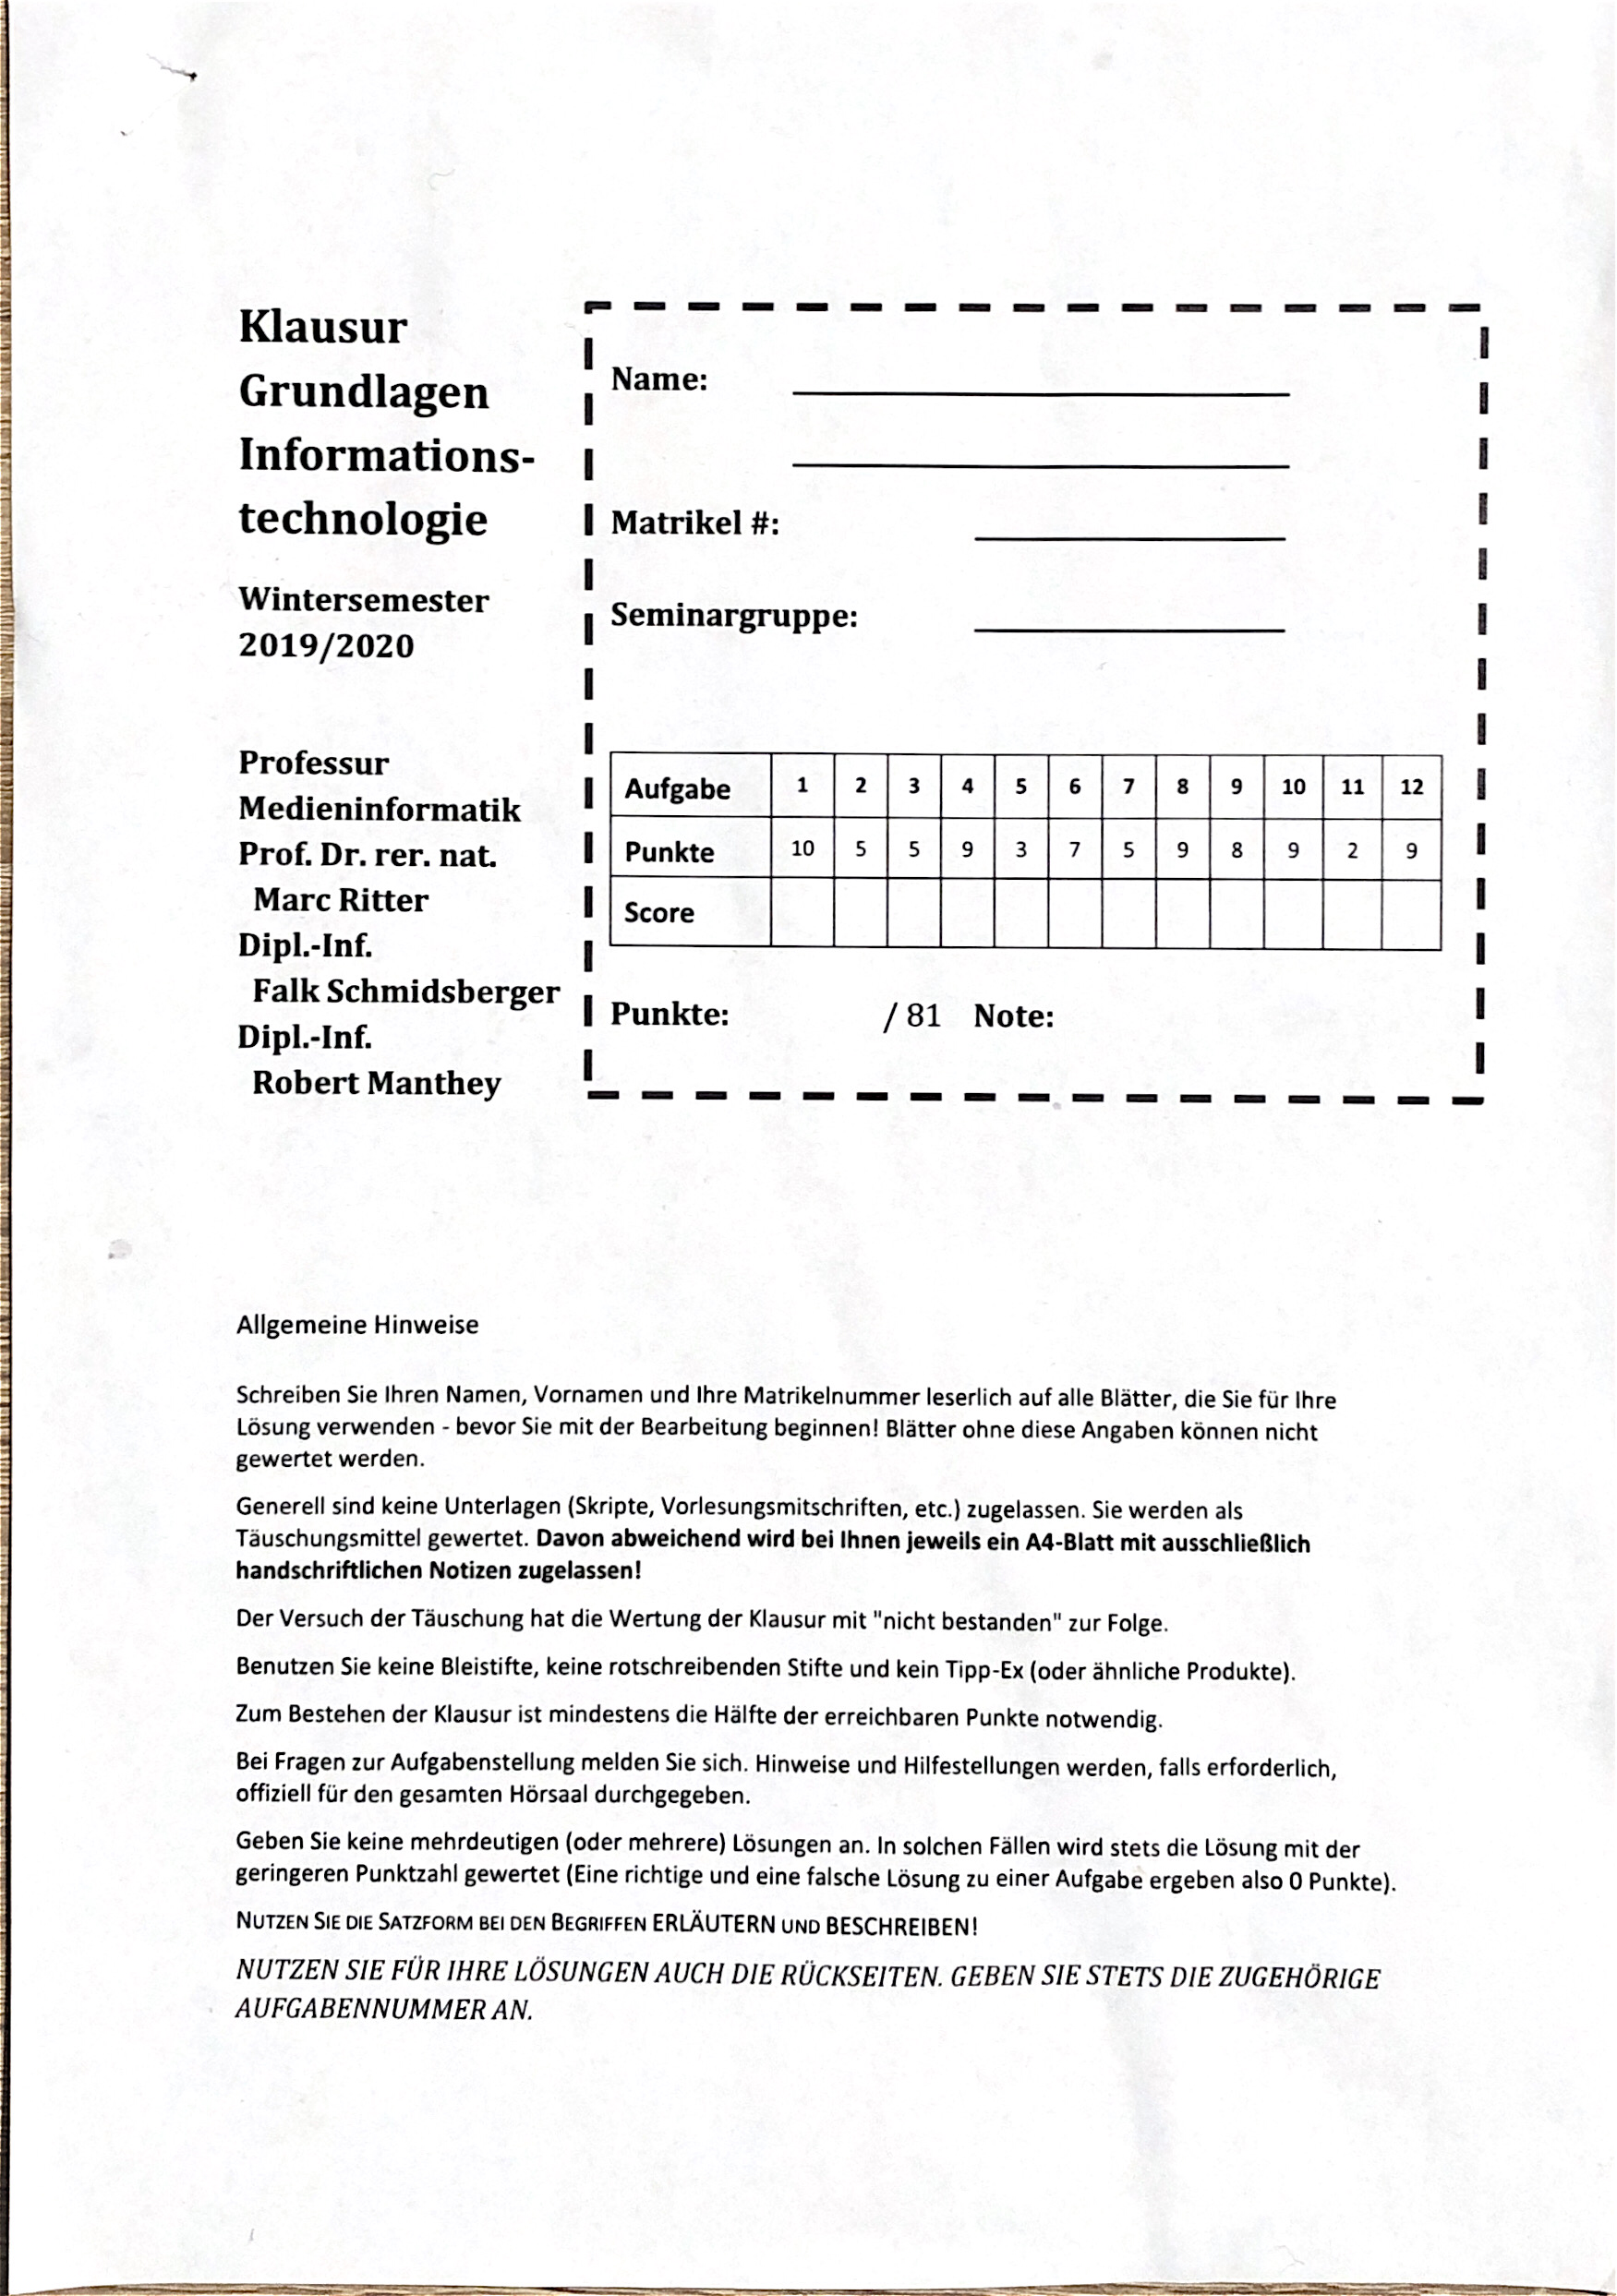
\includegraphics[width=0.96\textwidth]{img/seite1}}
        			\caption{Deckblatt der Klausur}
        			\label{fig:seite1}
    			\end{subfigure}
    			\begin{subfigure}[t]{0.4\textwidth}
        			\frame{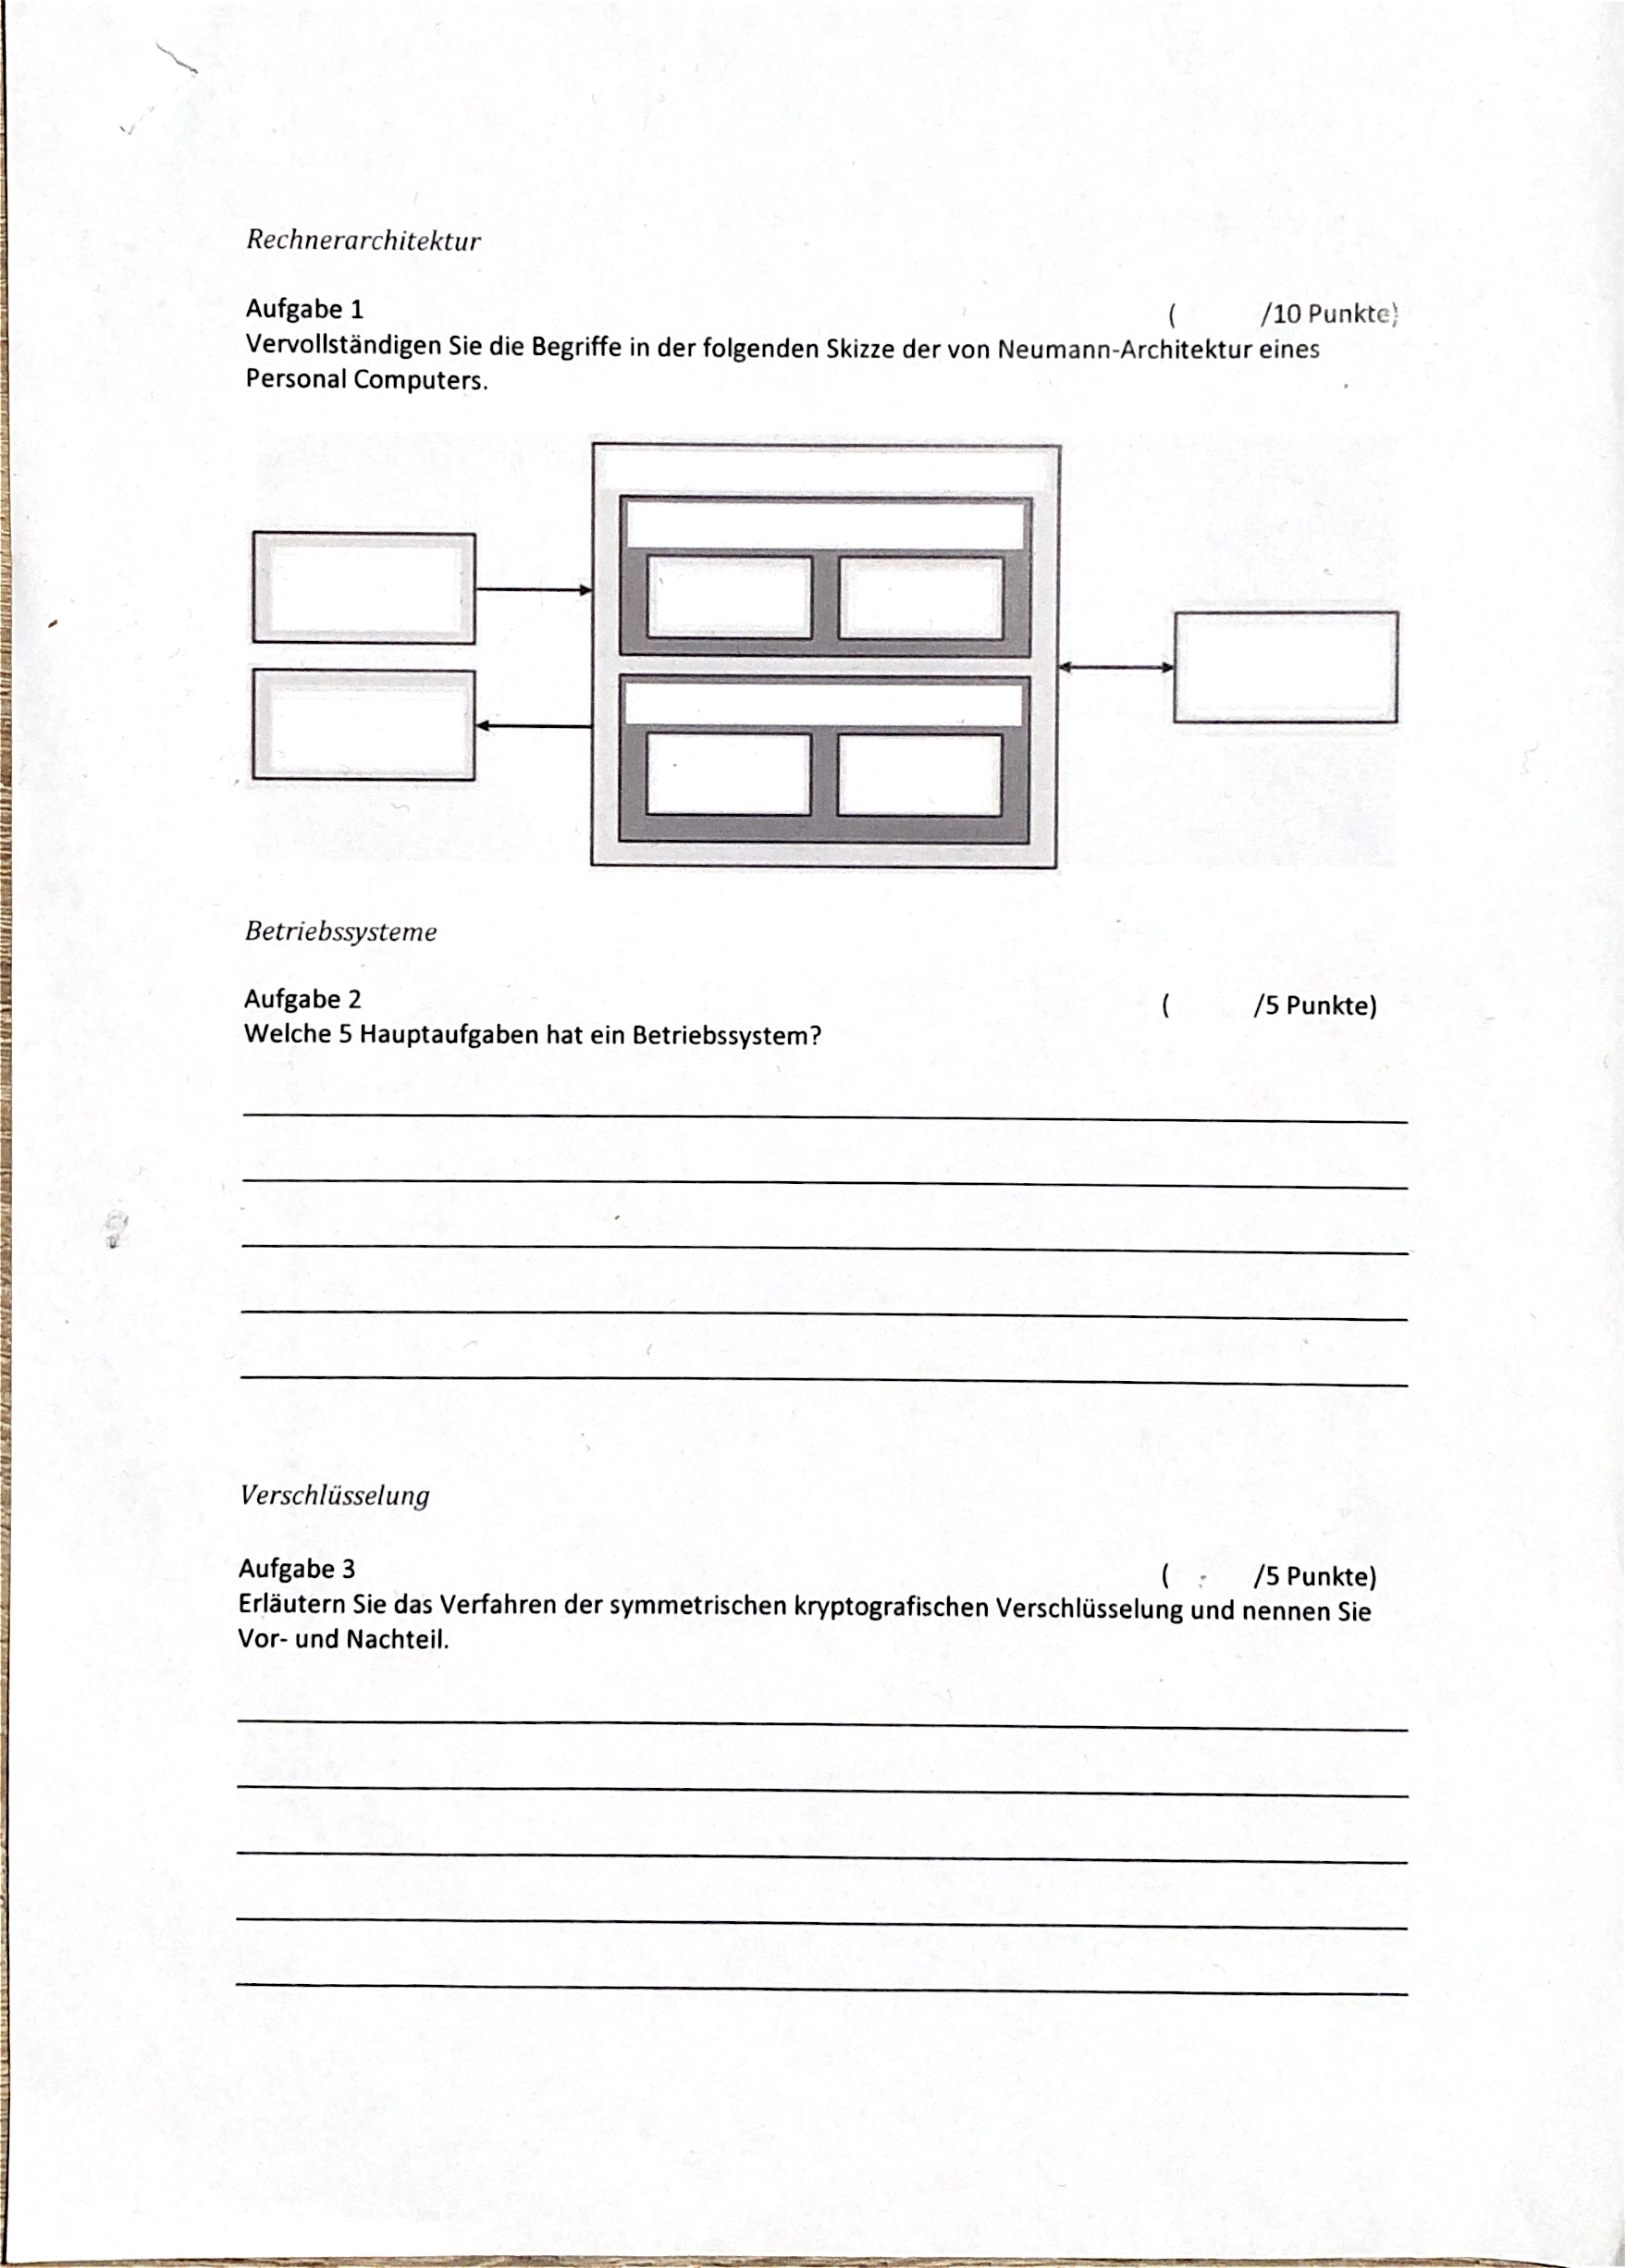
\includegraphics[width=0.96\textwidth]{img/seite2}}
        			\caption{1. Seite der Klausur}
        			\label{fig:seite2}
    			\end{subfigure}
    			\caption{Umsetzung der Klausuren-Vorlage der Fakultät CB.}
    			\caption*{\textit{Die Bilder sind beim Erstellen einer Scan-Vorlage mit der App entstanden.}}
    			\label{fig:klausur}
			\end{figure}
	
	Eine Klausuren-Vorlage bzw.\nomenclature{bzw.}{beziehungsweise} ein Gestaltungsleitfaden für Klausuren der Fakultät \textit{Angewandte Computer- und Biowissenschaften} bietet außerdem die Möglichkeit der Kontrolle des Prüfers an. Genauer ist es durch das vorgegebene Layout der Klausur möglich, einen Teil der Arbeit des Prüfenden auf Fehler zu untersuchen. Auf dem Deckblatt der Klausur ist eine Tabelle, mit drei Zeilen und für jede Aufgabe eine Spalte. In der ersten Zeile befinden sich die Nummern der Aufgaben. In der zweiten, die zu erreichenden Punkte der Aufgabe. Und in der dritten Zeile trägt der Prüfer die erbrachten Punkte des Studenten ein. Unter der Tabelle befindet sich ein Feld für die erreichte Gesamtpunktzahl, sowie ein Feld für die aus den Punkten resultierende Note. Die Punkte pro Aufgabe, die Gesamtpunktzahl und die Zensur stehen in Relation zu einander, sodass aus den Punkten der Aufgaben die beiden anderen Felder errechnet werden und mit den Ergebnissen des Prüfers abgeglichen werden könnten. Eine weiteres Merkmal der Klausuren-Vorlage ist ein Feld, für die vom Studenten erreichten Punkte über jeder Aufgabenstellung. Die dortige Angabe sollte mit der, in der Tabelle auf dem Deckblatt übereinstimmen und bietet somit noch eine weitere Möglichkeit der Kontrolle an.
	
	\section{Vorlage verbessern}
	Nachdem ein erster Prototyp zur Digitalisieren der Klausur-Daten entstanden ist, soll außerdem Prüfungsvorlagen entstehen, die für die Digitalisierung optimiert ist. Dabei sollen Probleme die beim Einscannen der aktuellen Vorlage erkannt wurden, behoben werden. 
	
	\section{Weitere Anmerkungen}
	Ferner soll bei der Lösung von der Anschaffung neuer Technologie und Geräte abgesehen werden. Grund dafür sind neben den Anschaffungskosten, die Idee, dass das Ergebnis des Forschungsprojekts in weiteren Lehr- und Forschungseinrichtung Anwendung finden sollte. Außerdem hat so gut wie jeder Mitarbeiter an einer Lehr- und Forschungseinrichtung ein eigenes oder Zugang zu einem Smartphone oder Tablet, welche durch die eingebaute Technik in der Lage sind, diese Aufgabe zu übernehmen. 

%%%%%%%%%%%%%%% - ANFORDERUNGEN - %%%%%%%%%%%%%%%

\chapter{Anforderungen}\label{ch:anforderungen}
	Es soll eine iOS-App entstehen mit der Klausuren digitalisiert werden können. Genauer müssen die, für die Notenfreigabe relevanten Daten der Klausur, in ein tabellarisches Format gebracht werden. Um unterschiedliche Klausuren oder auch andere Dokumente zu unterstützen, soll das Anlegen von Scan-Vorlagen in der App möglich sein. Hierfür (aber auch zum Einscannen) benötigt die App die Berechtigung für das Kamera-System. Diese muss, bei der ersten Benutzung einmalig erteilt werden.
	
	- Bild Scan-Vorlage: Aus Foto wird Dokument extrahiert und Auf der Seite werden Regionen markiert. -> Sammlung an Seiten mit Regionen
	
	Eine Scan-Vorlagen bestehen aus zwei Komponenten. Die eine sind zugeschnittene Fotos der Seiten eines Dokuments (\ref{fig:klausur}). Und die zweite sind die Regionen auf den Bildern, wo sich die zu digitalisierenden Informationen befinden. Dem Benutzer muss es möglich sein, zuerst die Fotos zu machen und anschließend Regionen auf den Seiten zu markieren. Weiter benötigen die Regionen Namen bzw. Typen, die der Benutzer angeben muss. Die Angabe des Typs ist wichtig, da dadurch eindeutig wird, ob es sich um die Note oder die Matrikelnummer des Studenten handelt. Diese Eindeutigkeit wird nicht nur für die automatische Erstellung der Tabelle benötigt, sondern auch für die Texterkennung. 
	
	Optical character recognition (OCR)\nomenclature{OCR}{optical character recognition, deutsch: optische Zeichen Erkennung und im deutschen Synonym für Texterkennung}, auf deutsch optische Zeichen Erkennung, soll dazu benutzt werden, die Informationen der Regionen zu digitalisieren. Um die Texterkennung zu verbessern, soll der Typ der Regionen verwendet werden. Damit könne dem OCR mögliche Ergebnisse mitgeteilt oder die Ergebnisse angepasst werden. Beispielsweise bestehen Zensuren immer aus Dezimalzahlen von Eins bis Sechs und mit nur einer Nachkommastelle. Wird der Buchstabe O anstelle der Ziffer Null erkannt, kann so der Fehler korrigiert werden.
	
	Zudem muss die Texterkennung auf dem Gerät selbst statt finden. Allerdings darf die App auch Texterkennung auf externen Servern unterstützen. Hierfür müssen dann die entsprechenden API-Schnittstellen implementiert oder für einen eigenen Server entwickelt werden.

	Die digitalisierten Daten, die für die Texterkennung entstandenen Dokumenten-Bilder und die erstellten Scan-Vorlagen, soll außerhalb der App auf einem Server gespeichert werden. Somit ist die Möglichkeit gegeben, die Vorlagen wieder zu verwenden und anderen Benutzern der App zur Verfügung zu stellen. Des Weiteren hat diese zentralen Stelle den Vorteil alle anfallenden Daten zu verwalten, was die Benutzung der App trotz vieler Benutzer vereinfacht.
	
	Damit Synchronität der Daten auf den Geräten und dem Server gewährleistet werden kann, benötig die App hierfür ebenfalls Schnittstellen. Diese sollten den standardmäßigen \textit{CRUD}\nomenclature{CRUD}{Das Akronym CRUD steht für Create/Erstellen, Read/Lesen, Update/Aktualisieren und Delete/Löschen und umfasst die vier grundlegenden Operationen persistenter Speicher}-Operationen entsprechen. 
	
	Da die gesamte Kommunikation über das Internet geschieht, muss das Softwaresystem die üblichen Datenschutz- und Datensicherheit-Richtlinien entsprechen, bzw. implementieren. 

%%%%%%%%%%%%%%% - GRUND IDEE ZUM LÖSEN DES PROBLEMS - %%%%%%%%%%%%%%%

\chapter{Konzept der Dokumenten-Scanner-App}\label{ch:konzept}

	Wie in der Problemstellung und Anforderung beschreiben, soll die Dokumenten-Scanner App wichtigen Daten auf dem Deckblatt einer Klausur, wie Vor- und Nachname des Studenten, seine Matrikelnummer sowie die Note erkennen, digitalisieren und in ein für die Notenfreigabe geeignetes Format bringen. Die digitalisierten Daten sollen anschließend an einen Server gesendet werde, wo sie und die beim Einscannen entstandenen Bilder gespeichert werden. Verwendet eine einzuscannende Klausur die Klausuren-Vorlage der Fakultät CB oder ähnliche, die eine Punkteübersicht haben, dann soll es außerdem möglich sein, die Punkte sowie die Note auf Richtigkeit zu überprüfen. 

	Zur Digitalisierung und Kontrolle der Daten werden Scan-Vorlagen verwendet. Diese muss vor dem Einscannen der ausgefüllten Klausuren erstellt werden, um zu gewährleisten, dass die richtigen Daten digitalisiert werden. Beim Erstellen einer Scan-Vorlage geht man wie folgt vor:
	\begin{itemize}
		\item Zuerst wird jede Seite der Klausur fotografiert (\ref{fig:v3}). Dabei wird in jedem Bild das Dokument erkannt, vom Hintergrund getrennt oder genauer gesagt ausgeschnitten und perfekt ausgerichtet (\ref{fig:klausur}). Zudem wird der Kontrast erhöht, so dass die Schrift leichter lesbarer wird.
		
		\item Anschließend markiert man diejenigen Regionen auf jeder Seite, die zu digitalisieren und/oder kontrollieren sind (\ref{fig:v9}). Zusätzlich muss jeder Region ein Name und einer der folgenden Typen zugeordnet werden: Unbekannt, Name, Matrikelnummer, Seminargruppe, Punkte und Note. Mithilfe des Typs wird die Texterkennung verbessert und falsche Ergebnisse automatisch korrigiert. Dazu später mehr.
			
		\item Des Weiteren kann man aus allen markierten Regionen diese auswählen, die in Relation stehen. Diesen Relationen werden danach noch weitere Eigenschaften zugeteilt, um sie später bei der Kontrolle richtig zu analysieren. So eine Eigenschaft könnte sein, dass es sich um einen Vergleich zwischen zwei in Relation stehenden Regionen handelt. Z. B. ist die eine Region die Zelle in der Punkteübersichts-Tabelle, in der die erreichten Punkte zu Aufgabe 1 rein geschrieben werden sollen. Und die zweite Region die Stelle über der Aufgabenstellung von Aufgabe 1, in der ebenfalls die erreichten Punkte eingetragen werden sollen. Weitere Beispiele für solche Relationen und Eigenschaften sind die Summanden für die erreichte Gesamtpunktzahl und die Summe selbst, oder auch noch die daraus resultierende Note.
		
		\item Als letztes speichert man die Vorlage ab, welche dann automatisch an einen Server gesendet wird, so dass andere diese Vorlage ebenfalls nutzen können.
	\end{itemize}
	
	Nach der Erstellung einer Vorlage kann das Dokument digitalisiert werden. Dazu scannt man die Seiten in derselben Reihenfolge, wie in der Scan-Vorlage ein. Die App digitalisiert mithilfe von OCR den Inhalt, in den vordefinierten Regionen. Der Typ der Region nimmt nun Einfluss auf das Ergebnis. Durch ihn wird während der Worterkennungsphase eine Liste an vordefinierten möglichen Ergebnissen eingespeist. Diese Liste hat Vorrang vor dem Standard-Lexikon und verbessert dadurch die Texterkennung. Ein Beispiel für solch eine Liste könnten, alle möglichen Noten sein, wie schon in dem Kapitel \ref{ch:anforderungen} Anforderungen beschrieben. Auch vorstellbar ist, dass alle Seminargruppen oder Namen von Personen, die an der Klausur teilgenommen haben, dort verwendet werden. 
	
	Weiter wäre eine zusätzliche Möglichkeit der Korrektur erdenklich. Angenommen, jemand verschreibt sich bei seiner Seminargruppe und vergisst ein Zeichen. Die Texterkennung erkennt zwar jedes Zeichen richtig, jedoch ist das Ergebnis keine korrekte Seminargruppe. Deshalb könnte man auch im Nachhinein das Ergebnis mit einer Seminargruppe ersetzt, die die größte Übereinstimmung mit dem erkannten Wort hat. Bei diesem Vorgehen sollten natürlich auch nur die Seminargruppen verwendet werden, die tatsächlich die Klausur geschrieben haben. Ähnliches gilt wieder für die Namen oder Matrikelnummern der Studenten.
	
	Zudem kommt noch, dass die eingetragenen Punkte kontrolliert werden. Möglich wäre auch, die Note zu kontrollieren, jedoch müsste dafür der jeweilige Notenspiegel integriert werden. Für die Umsetzung dieser Kontrollinstanz werden die angelegten Relationen zwischen den Regionen verwendet. Genauer soll es zwei Typen von Links bzw. Relationen geben.
		\begin{itemize}
			\item Der erste Typ ist zum Vergleichen. Dafür benötigt es genau zwei Regionen und wie der Name des Typs ahnen lässt, wird der Inhalt der beiden Regionen auf Gleichheit überprüft. Wie schon vorher erwähnt, sollen so die Punkte auf dem Deckblatt mit den Punkte über den Aufgaben verglichen werden.
			\item Der zweite Typ ist zum Summieren. Genauer ist dieser Typ nur für die Punkte auf dem Deckblatt der Klausur gedacht. Dabei wählt man alle Regionen aus, deren Inhalt summiert werden sollen und die Region, in die der Prüfer die berechnete Gesamtpunktzahl rein schreibt. Somit kann die Berechnung des Prüfers überprüft werden.
		\end{itemize} 
		Mithilfe der beiden Typen, wird dem Benutzer nach der Texterkennung mitgeteilt, wo Fehler vorliegen.
		
	Allerdings heißt das nicht, dass das OCR selbst keine Fehler macht. Aus diesem Grund ist die sogenannte confidence des OCR bei jeder Region sichtbar. Diese sagt aus, wie sicher sich die Texterkennung ist, das das Ergebnis stimmt. Jedoch kann es auch hier falsche Positiv-Ergebnisse geben, weshalb auch das kein perfekter Indikator für die Richtigkeit ist. Deshalb wird im Anschluss an die Texterkennung die Möglichkeit geboten, die Resultate noch einmal zu überprüfen und zu korrigieren, bevor sie an den Server zum Abspeichern gesendet werden. Genauer können die Ergebnisse der Texterkennung zu jeder Region einzeln bearbeitet werden, wodurch sich die Fehlermeldung durch einen Link ändern kann.

%%%%%%%%%%%%%%% - PROTOTYP - %%%%%%%%%%%%%%%

\chapter{Entwicklung des ersten Prototyps}
	Dieses Kapitel beschreibt die Entwicklung der iOS-App in einer ähnlichen Reihenfolge, wie das bekannte Wasserfall-Model über die Verwaltung der Entwicklung großer Softwaresysteme nach Winston W. Royce. - Quelle:...
	
	\section{Anforderungsplanung}
	Vor Beginn des Praktikums wurde diskutiert und kalkuliert, welches Thema aus dem Projekt Memo Space für ein zwölfwöchiges Praktikum geeignet ist. Dabei entstand eine Art Durchführbarkeits- / Machbarkeitsstudie, welche zur Entscheidung führte, ein Dokumenten-Scanner-Softwaresystem umzusetzen. Aufgrund der Kenntnisse und Erfahrung, soll ein Backend mit entsprechenden Schnittstellen und einer Android-App von Tobias Kallauke umgesetzt werden, währende vom Verfasser eine iOS-App gefordert ist. Die Anwendung soll den Anforderungen, die im gleichnamigen Kapitel \ref{ch:anforderungen} zu finden sind, erfüllen. Für weitere Details über den Server und die Android-App siehe im Praktikumsbericht von Tobias Kallauke.

	\section{Planung und Vorbereitung bzw. Analyse und Definition}
		Die Aufgaben bzw. Ziele dieser Phase sind:
		\begin{enumerate}
			\item die Auseinandersetzung mit der Problemstellung und den Anforderungen,
			\item das Betreiben von einer Problemanalyse,
			\item die Entwicklung von Ideen und eines genauen Konzepts der iOS-App sowie 
			\item das Entwickeln eines ersten Prototyps, als Machbarkeitsnachweis.
		\end{enumerate}
		
		Bei der Entstehung des Konzepts, welches im Kapitel \ref{ch:konzept} zu finden ist, spielen die Dokumentationen der Frameworks \textit{Vision}, \textit{VisionKit} und \textit{PhotoKit} von \textit{Apple} eine entscheidende Rolle. Aus ihnen wird klar, welche Funktionen der App noch zu entwickeln und welche in Frameworks schon vorhanden sind. Z. B. ist das Erkennen und das gerade Ziehen von Dokumenten in Echtzeit, sowie die Texterkennung auf Bildern in \textit{Vision} und \textit{VisionKit} enthalten. Bei der Entwicklung des ersten Prototyps half eine Beispiel-App von \textit{Apple} \cite{noauthor_detecting_nodate}, die das Erkennen von Objekten in Standbildern mithilfe der genannten Frameworks umsetzt.
		
		Durch die Auseinandersetzung mit den Bibliotheken konnte festgestellt werden, dass die zu entwickelnde App nur Geräte mit iOS 13.0 oder neuer unterstützen werden kann. Grund dafür sind die \textit{Apple} Frameworks \textit{SwiftUI} und \textit{VisionKit}. \textit{SwiftUI} bietet die Möglichkeit, Benutzeroberflächen für alle \textit{Apple}-Plattformen in \textit{Swift} zu erstellen. Die deklarative \textit{Swift}-Syntax ist einfach zu lesen und schnell zu schreiben, so dass es möglich ist, die App in wenigen Wochen für iPhone und iPad zu schreiben. Als Alternative gibt es noch \textit{UIKit} oder auch \textit{AppKit}, die unter alle iOS Versionen funktioniere. Diese Frameworks sind allerdings nicht deklarativ sodass, Views sowohl im Code als auch in Interface-Dateien getrennt voneinander erstellt und konfiguriert werden müssen \cite{sillmann_einstieg_nodate}. Dadurch dauert die Entwicklung einer App, im Gegensatz zu SwiftUI deutlich länger, wie man auch hier in dem Video \footnote{SwiftUI vs UIKit – Comparison of building the same app in each framework - \href{https://www.youtube.com/watch?v=qk2y-TiLDZo}{\url{https://www.youtube.com/watch?v=qk2y-TiLDZo}} } von Paul Hudson einem in der Swift-Community sehr bekannten Programmiere und Autor sieht. Sehr ähnliche Erfahrung hat der Verfasser vor dem Praktikum mit den beiden Frameworks gemacht. \textit{VisionKit} dagegen, ist das Framework zum Scannen der Dokumente. Auch hierfür gibt es eine Alternative. Das Framework ist von den Entwicklern von \textit{WeTransfer} und funktioniert auch auf älteren iOS Versionen. Allerdings unterstützt \textit{WeScan} \footnote{WeScan GitHub Repository - \href{https://github.com/WeTransfer/WeScan}{\url{https://github.com/WeTransfer/WeScan}}} noch kein stapelweises Scannen. Das bedeutet, man kann immer nur ein Foto machen, welches erst abgespeichert werden muss, bevor man das nächste machen kann. Das ist für den Benutzer nicht bequem und spart wahrscheinlich auch keine Zeit.

		Abschließend zu dieser Phase ist zu erwähnen, dass das Scrum-Konzept, welches sich für agile Softwareentwicklung anbietet, zur Projektplanung und zum Projektmanagement verwendet wurde. Als Versionsverwaltung der Software wurde Git in Kombination mit GitHub Issues und GitHub Projects als Planungstools benutzt. So konnte der Verfasser selbständig jedem Sprint Aufgaben zuordnen und den Fortschritt nachvollziehen.

	\section{Grundlagen}
			In den folgenden zwei Absätze werden wichtige Konzepte und Grundwissen vermittelt, die im folgenden Kapitel Entwurf und Design nochmal aufgegriffen werden.

		\paragraph{Model-View-ViewModel:}
			Das Entwurfsmuster Model View ViewModel (MVVM)\nomenclature{MVVM}{Model View ViewModel} entstand bei \textit{Microsoft} im Jahr 2005 mit der \textit{Windows Presentation Foundation} (WPF) und \textit{Silverlight-Technologien}. MVVM verwendet das Konzept eines Schichtmodells und ist eine abstrakte Darstellung einer Benutzeroberfläche, in Form einer Klasse, wie man sie unter objektorientierten Programmiersprachen kennt. Diese Klasse enthält Daten, die auf der Benutzeroberfläche angezeigt werden sollen und Anweisungen, die auf der Benutzeroberfläche aufgerufen werden können. Dieses sogenannte ViewModel, weiß nichts von Views, wie es sonst bei anderen Entwurfsmustern üblich ist, um Daten auf der Benutzeroberfläche anzuzeigen. Stattdessen verwendet eine MVVM-View eine Bindungsfunktion (data binging) zur bidirektionalen Zuordnung von Daten aus dem ViewModel zu den jeweiligen Eigenschaften auf der View. Z. B. Einträge in einer Dropdown-Menü. Aber auch das binden von Daten aus dem Model zu Benutzereingaben durch Maus, Tastatur oder Touch-Screens ist möglich. Beispielsweise kann ein Mausklick eine Anweisung in dem ViewModel auslösen. Diese verändert einen Wert im Model, wodurch die View durch data binding aktualisiert wird. \cite{freeman_pro_2017} \cite{bragge_model-view-controller_2013}

		\paragraph{Redux.js:}
			Redux.js ist eine Bibliothek\footnote{Redux.js Github Repository - \href{https://github.com/reduxjs/redux}{\url{https://github.com/reduxjs/redux}}} für die Programmiersprache JavaScript. Diese stellt einen sogenannten vorhersehbaren Zustandscontainer\footnote{Core Concepts - \href{https://redux.js.org/introduction/core-concepts}{\url{https://redux.js.org/introduction/core-concepts}}} für JavaScript Anwendungen bereit. In diesem Container wird der Zustand der gesamten Anwendung in einem Objektbaum innerhalb eines einzigen Speichers gespeichert. Diesen Baum kann man sich vorstellen, wie eine Matrjoschka die weitere Puppen in sich hat. Der wichtige Unterschied zwischen einer Matrjoschka und einem Baum ist jedoch, dass in eine Puppe genau nur eine andere gesteckt werden kann. Beim einem Objektbaum hingegen können mehrere Objekte in ein Objekt ''gesteckt'' werden und so weiter. Im Bezug auf einen Zustandscontainer enthält dieser dann States (Objekte) auf deutsch Zustände und Daten, die unteranderem auf der Benutzeroberfläche angezeigt werden sollen. Diese Aufteilung in die States ist dazu gedacht, einer View oder mehrere zusammenhängende Views nur die wirklich benötigten Daten bereit zustellen. Diese Struktur erleichtert das Testen oder Untersuchen der Anwendung und ermöglicht es, durch hinzufügen eines neuen States den aktuellen Entwicklungsstand der Anwendung beizubehalten und dadurch den Entwicklungsprozess zu beschleunigen. \\
			Ein weiteres wichtiges Prinzip\footnote{Three Principles - \href{https://redux.js.org/introduction/three-principles}{\url{https://redux.js.org/introduction/three-principles}}} von Redux ist, dass die Daten in den States Schreibgeschütz sind. Die einzige Möglichkeit den Zustand zu ändern, besteht darin, eine Aktion auszulösen, die beschreibt, was passiert. Dadurch wird sichergestellt, dass weder die Views noch Netzwerk-Rückrufe jemals direkt an den Zustand schreiben werden. Stattdessen bringen sie nur die Absicht zum Ausdruck, den Zustand zu verändern und lösen eine Aktion aus. Da alle Änderungen zentralisiert sind und eine nach der anderen in einer strikten Reihenfolge erfolgen, gibt es weniger Programmfehler-Quellen.

	\section{Entwurf und Design}

		- Quelle Schubert Folien
		
		Eine typische Aufgabe dieser Entwurfsphase ist die Entscheidung über die Datenhaltung, die Verteilung im Netz und die Benutzeroberfläche des Software-Systems. Jedoch standen diese Grundsatzentscheidungen schon zu Beginn des Praktika, durch die Kenntnisse von Tobias Kallauke und dem Verfasser fest. Der Server verwendet zur Datenspeicherung Postgres, eine relationale Datenbank, sowie das Dateiverzeichnis für Bilder, während die App keine Daten persistent speichert. Durch die Aufteilung von App und Server handelt es sich um eine sogenannte Client/Server-Architektur und für die Benutzeroberfläche wird das deklarative SwiftUI verwendet. Bei Fragen zum Backend und der Android App siehe im Praktikumsbericht von Tobias Kallauke.
		
		Jedoch mussten noch Arbeit in den Workflow und in die Architektur der App gesteckt werden. Zur Definition einzelner Teil-Workflows, die zusammenhängende Aufgaben umfassen, wurden eine Art Zustandsautomaten bzw. Flussdiagramm beschrieben. Ein Beispiel, was noch einmal geändert in der App verwendet wurde befindet sich im Anhang \ref{ch:workflow}. Die Modelle halfen dabei Views zu entwickeln und deren Design festzulegen. Das Aussehen der App sollten sich jedoch im Laufe der Zeit noch ändern, denn ersteinmal stand die Umsetzung des Konzepts im Vordergrund.

		Aus den Designs und den Teil-Workflows heraus entstand ein grober Plan, wie die Daten in der App gehandhabt werden sollten. Da \textit{SwiftUI} das Entwurfsmuster MVVM umsetzt, benötigt es eine Struktur für das ViewModel und für den Datenfluss der asynchronen Server-Rückrufe. Jedoch stellte sich die Entwicklung dieser Strukturen, auch schon während des allerersten Prototyps, als problematisch heraus. Denn auch bei steigender Komplexität soll das ViewModel noch übersichtlich bleiben, um eine schnelle Weiterentwicklung zu gewährleisten. Aus diesen Gründen begann die Suche nach einer besseren Lösung, bei der die JavaScript-Bibliothek \textit{Redux.js} zur Verwaltung von Zustandsinformationen in Webanwendung entdeckt wurde. 

		\textit{Redux} hilft durch dessen Konzept, komplexe Views mit vielen Daten schnell und einfach zu implementieren. Auch werden so Serverantworten und zwischengespeicherte Daten sowie lokal erstellte Daten, die noch nicht auf dem Server gespeichert wurden, strukturiert und zentral abgelegt. Das erleichtert nicht nur das Wiederverwenden von Daten, sondern spart auch wiederholte Server-Aufrufe ein. Es erschien nun möglich, trotz der begrenzten Zeit im Praktikum, möglichst viel mit wenig Fehlern umzusetzen. Denn Redux ermöglicht durch die modulare Aufteilung des State Containers eine schnelle Weiterentwicklung der App, auch wenn die Komplexität der Anwendung steigt. Und die Vorteile von Redux hinsichtlich des Testens und Untersuchens der App sollten helfen, Fehler möglichst schnell ausfindig zu machen, trotz asynchroner Programmabschnitte.

		Daher lag es nah die wesentlichen Konzepte von \textit{Redux} umzusetzen und einen \textit{Redux} ähnlichen State Container, als ViewModel zu implementieren. Aus der Definition von Teil-Workflows sollte der Container oder auch Store genannt mindestens 5 States haben: 
		\begin{itemize}
			\item für Authentifizierung sowie Registrierung,
			\item für das Anlegen von Vorlagen, um Zwischenergebnisse zu speichern,
			\item für das Ausführen von Server-Aufrufen zum Speichern und Abrufen von Vorlagen, 
			\item für die Steuerung des Workflows bzw. den stellvertretenden Views sowie
			\item für sonstige Daten, die sehr häufig verwendet werden.
		\end{itemize}
		
		\begin{figure}[th]
			\centering
			\begin{subfigure}[t]{0.48\textwidth}
				\centering
				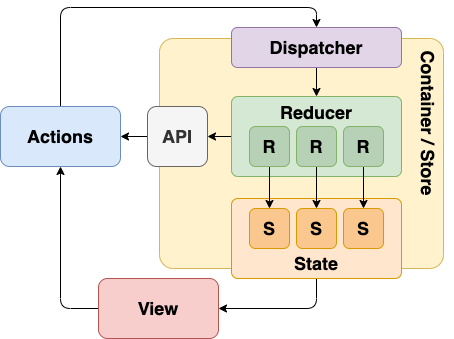
\includegraphics[width=\textwidth]{img/redux.png}
				\caption{Schema der Documenten-Scanner Architektur}
				\label{fig:redux}
			\end{subfigure}
			\begin{subfigure}[t]{0.48\textwidth}
				\centering
				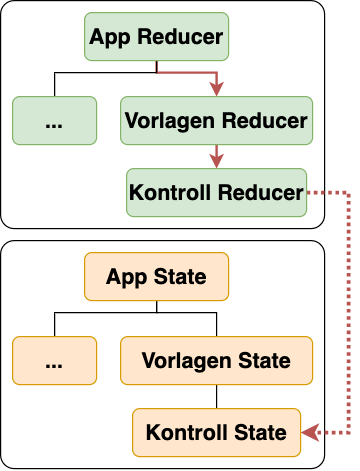
\includegraphics[height=0.9\textwidth]{img/tree_example.png}
				\caption{Reducer- und State-Objektbaum}
				\label{fig:tree}
			\end{subfigure}
			\caption{Architektur Schemata}
		\end{figure}
		
		Das Schema \ref{fig:redux} zeigt, die in der App umgesetzte Redux ähnliche Struktur. Über eine View (rot) können Aktionen (blau) aufgerufen werden. Diese gelangt zuerst in einen sogenannten Dispatcher (lila), welcher als Verteiler dient. Anhand der Art einer Aktion, wird der entsprechende Reducer (grün) vom Dispatcher beauftragt, die Aktion auszuführen. Ein Reducer ist für genau eine Art von Aktionen zuständig. Allerdings ist, wie in der Abbildung \ref{fig:tree} zu sehen ist, eine Schachtellung von Reducern (grün) möglich. Dies bedeutet auch, dass Aktions-Arten ineinander geschachtelt werden können. Das hat den Hintergrund, dass die States wie ein Objektbaum aufgebaut sind. So hat jeder State seinen eigenen Reducer, was für die oben erwähnte Modularität sorgt. Möchte man beispielsweise eine Änderung im Link State (siehe \ref{fig:tree}) vornehmen, muss die eigentliche Aktion in einer Link Reducer Aktion gekapselt und diese wiederum in einer Vorlagen Reducer Aktion. Zum ausführen der Aktion, werden dann die entsprechenden Reducer die Kapselung von außen nach innen auflösen. Nachdem die Aktion ausgeführt und eine State-Änderung herbeigeführt wurde, aktualisiert sich durch das data binding von MVVM die View. Genauer werden alle Views, die eine Bindung zu dem geänderten Datum haben, über die Änderung benachrichtigt und daraufhin aktualisieren diese sich.

		Ein weiterer wichtiger Punkt sind die Server-Aufrufe. Für diese gibt es einen eigenen Reducer und eine besondere Schnittstelle, welche in der Abbildung \ref{fig:redux} grau markiert und mit API \nomenclature{API}{application programming interface, auf deutsch Programmierschnittstelle} beschriftet ist. Diese hat die Besonderheit selbst Aktionen an den Container zu senden. Beispielsweise löst ein Knopfdruck in einer View die Aktion aus, alle Vorlagen vom Server zu laden. Diese Aktion gelangt über den vorgesehenen Reducer zu der Schnittstelle. Dort wird ein entsprechender Server-Aufruf gestartet und ohne andere Prozesse anzuhalten auf den Server-Rückruf gewartet. Sobald die Antwort des Servers angekommen ist, wird diese in einer Aktion wieder zum Container gesendet. Dort wird sich wieder ein entsprechender Reducer um eventuelle Fehlerbehandlung oder das Ablegen der Vorlagen kümmern.
		
	\section{Implementierung}
		
		Zur Realisierung der entworfenen Systemkomponenten wurde ausschließlich, die von Apple entwickelte IDE\nomenclature{IDE}{integrated development environment, auf deutsch Integrierte Entwicklungsumgebung} Xcode, verwendet. Diese stellt Geräte-Simulatoren zur Verfügung, auf denen die App getestet werden kann. Die Simulatoren bieten unteranderem auch die Möglichkeit an, die Anwendung schnell auf verschiedenen iOS bzw. iPadOS Versionen zu testen. Auch ist das Testen der App auf echten Geräten durch Xcode möglich, was bei der Entwicklung unumgänglich war. Grund dafür ist die Benutzung der Kamera, die bei den Simulatoren zu gewollten Abstürzen führt, da diese keinen Zugriff auf eine Kamerasystem besitzen. 
		
		Zum Ändern und Testen des Backends wurde außerdem Visual Studio Community bzw. Visual Studio Code\footnote{\href{https://visualstudio.microsoft.com/de/}{\url{https://visualstudio.microsoft.com/de/}}} mit dem REST Client Plugin\footnote{\href{https://marketplace.visualstudio.com/items?itemName=humao.rest-client}{\url{https://marketplace.visualstudio.com/items?itemName=humao.rest-client}}} , zum Testen der Server-Schnittstellen verwendet. Das Backend konnte dann als lokaler Server auf dem Entwicklungscomputer gestartet und über die IP-Adresse 0.0.0.0 sogar im lokalen Netzwerk aufgerufen werden. Für die Verwaltung der PostgreSQL-Datenbank genügte das Tool PgAdmin4\footnote{\href{https://www.pgadmin.org/}{\url{https://www.pgadmin.org/}}} . Damit ist es möglich einzelne Einträge oder auch ganze Tabellen zu bearbeiten.
			
		\subsection{Registrieren und Anmelden}
			\begin{figure}[th]
    			\centering
    			\begin{subfigure}[t]{0.3\textwidth}
        			\frame{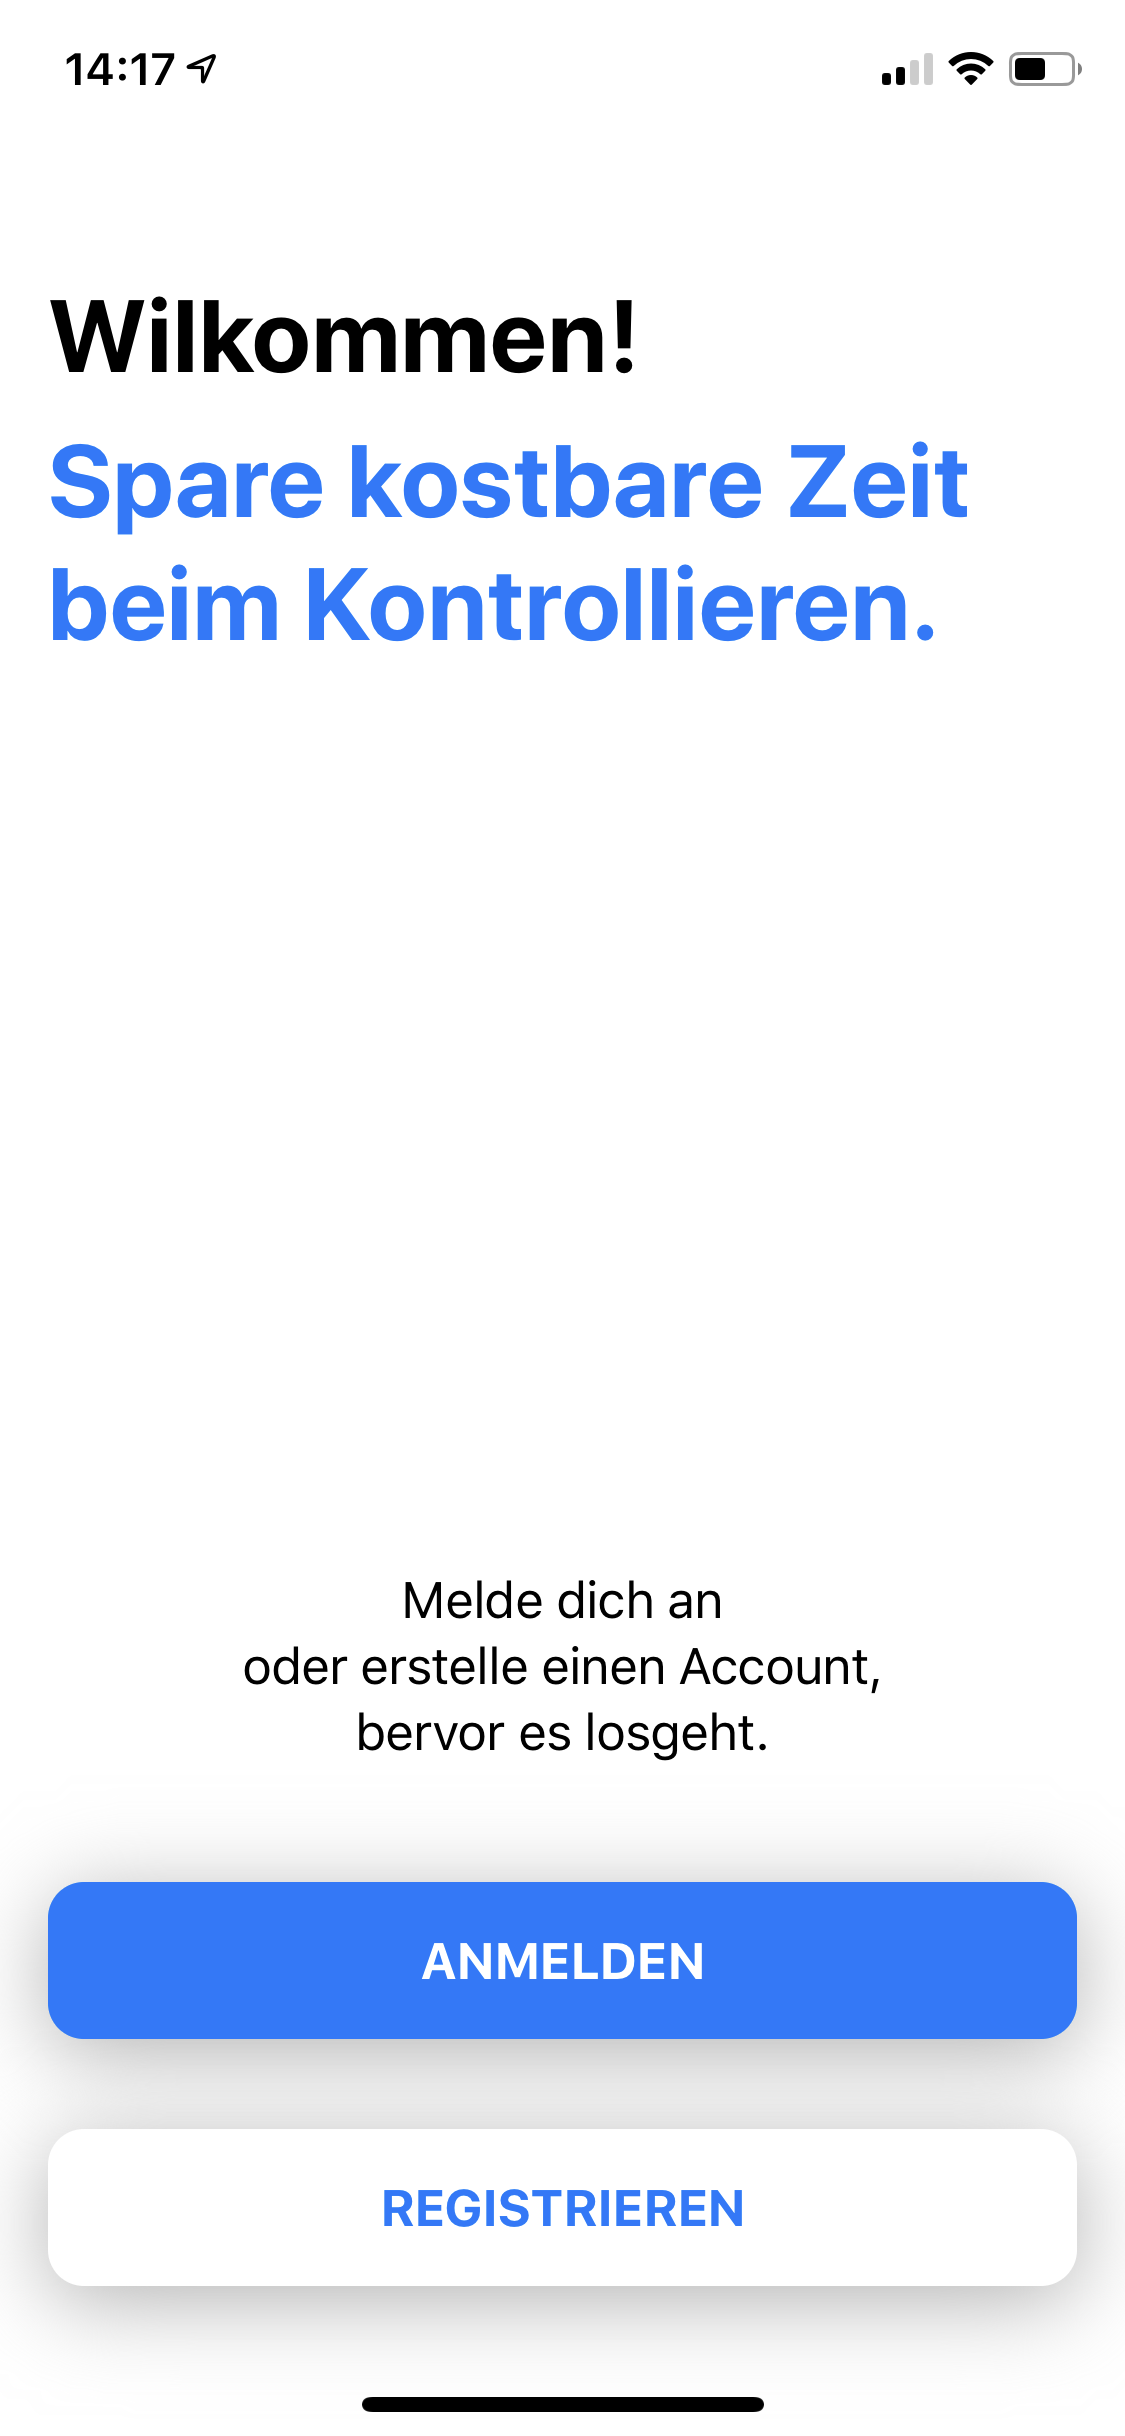
\includegraphics[width=0.96\textwidth]{img/1willkommen.png}}
        			\caption{Willkommen View}
        			\label{fig:willkommen}
    			\end{subfigure}
    			\begin{subfigure}[t]{0.3\textwidth}
        			\frame{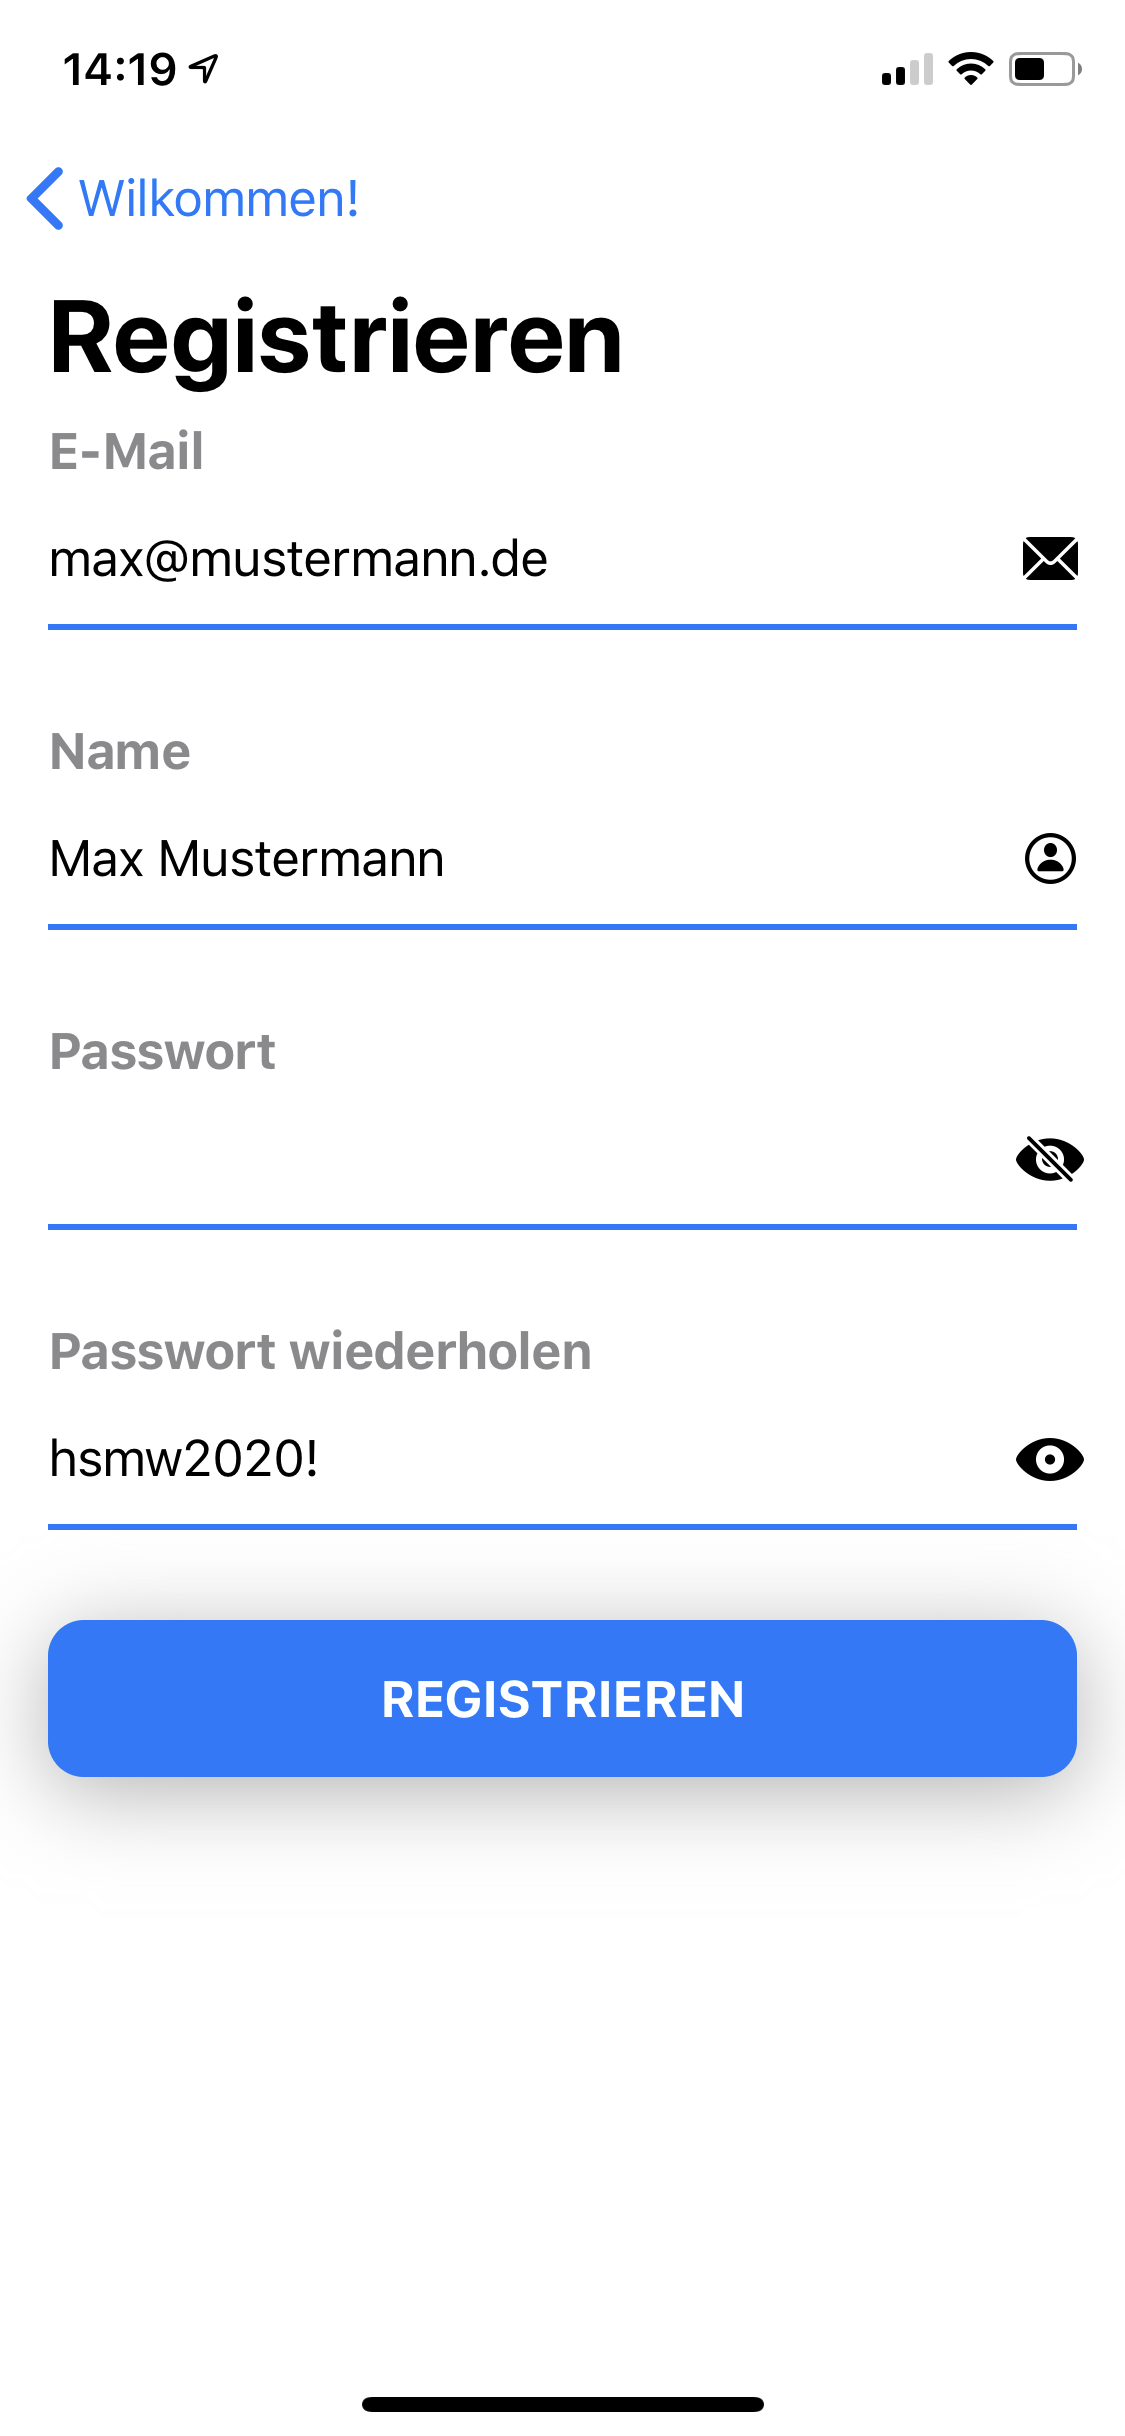
\includegraphics[width=0.96\textwidth]{img/7reg_full_see.png}}
        			\caption{Registrierung mit sicheren Eingabefeldern}
        			\label{fig:register}
    			\end{subfigure}
    			\begin{subfigure}[t]{0.3\textwidth}
       				\frame{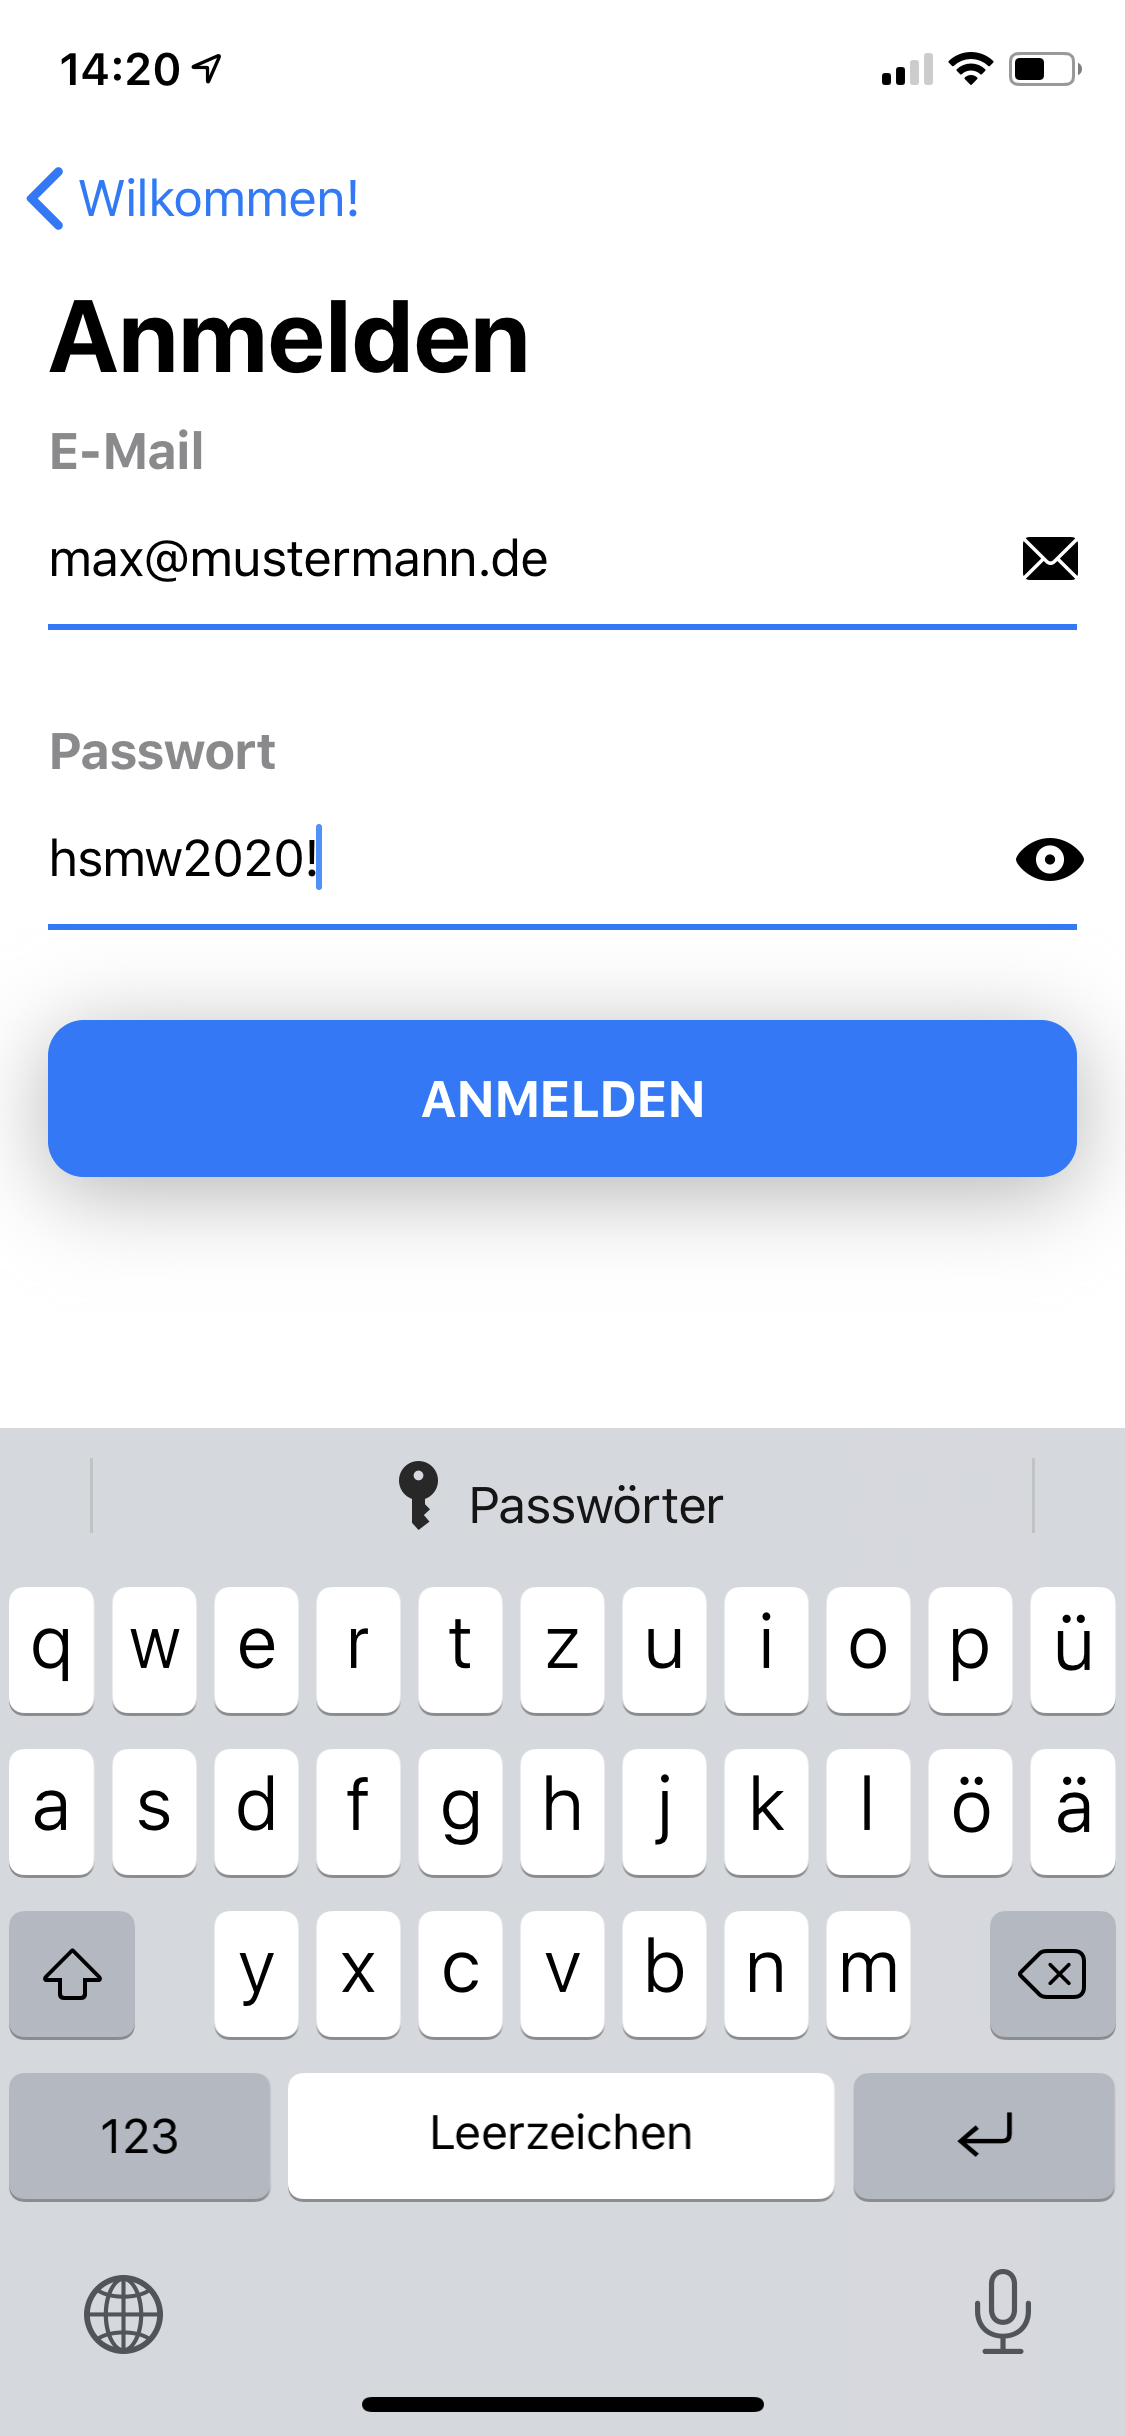
\includegraphics[width=0.96\textwidth]{img/12an_full_pass.png}}
        			\caption{Anmeldung mit AutoFill-Funktion}
        			\label{fig:anmelden}
    			\end{subfigure}
    			\caption{Willkommen- Registrier- und Anmelde-View}\label{fig:start}
			\end{figure}
			
			Die technische Implementierung der Registrierung und Anmeldung beinhaltet typische Charakteristiken von Anmelde- und Registrier-Formularen. Die E-Mail-Textfelder besitzen, wie auch das Passwort-Feld der Anmeldung eine AutoFill-Funktion. Dadurch kann das iOS-Gerät Registrier- und Anmelde-Daten vorschlagen und automatisch in die entsprechenden Felder einsetzten. Dies sieht man im dritten Bild \ref{fig:anmelden} anhand des ''Passwörter''-Knopfes über der Tastatur.  Weiter sind alle Passwort-Felder gesichert. Das bedeutet, dass der Inhalt zum Schutz der Privatsphäre standardmäßig ausgeblendet und mit Punkten ersetzt wird. Durch das drücken des Auges rechts des Textfeldes kann der Inhalt jedoch eingesehen werden. Im mittlerem Bild \ref{fig:register} sind wegen der Sicherheitsstandards von iOS, bei einer Aufnahme des Bildschirms nicht einmal die Punkte des ersten Passwort-Textfelds zu sehen. Zusätzlich validieren alle Text-Felder ihren Inhalt mithilfe von regulären Ausdrücken. Beispielsweiße muss ein Passwort aus 8 Zeichen bestehen und zwei von den drei Folgenden Eigenschaften erfüllen:
			\begin{enumerate}
				\item Es ist mindestens ein Sonderzeichen enthalten.
				\item Es ist mindestens ein Großbuchstabe enthalten.
				\item Es ist mindestens eine Zahl enthalten.
			\end{enumerate}
			Die Validierung ist jedoch nicht standardmäßig, sondern wurde selbst entwickelt.
			
		\subsection{Scan-Vorlagen erstellen und speichern}
			Bei der Implementierung des ersten Arbeitsschritts der Scan-Vorlagen wurde das schriftliche Flussdiagramm, welches im Anhang \ref{ch:workflow} zu finden ist, leicht verändert benutzt.
			
			\subsubsection{Scan-Vorlage erstellen}
			\begin{figure}[th]
    			\centering
    			\begin{subfigure}[t]{0.3\textwidth}
        			\frame{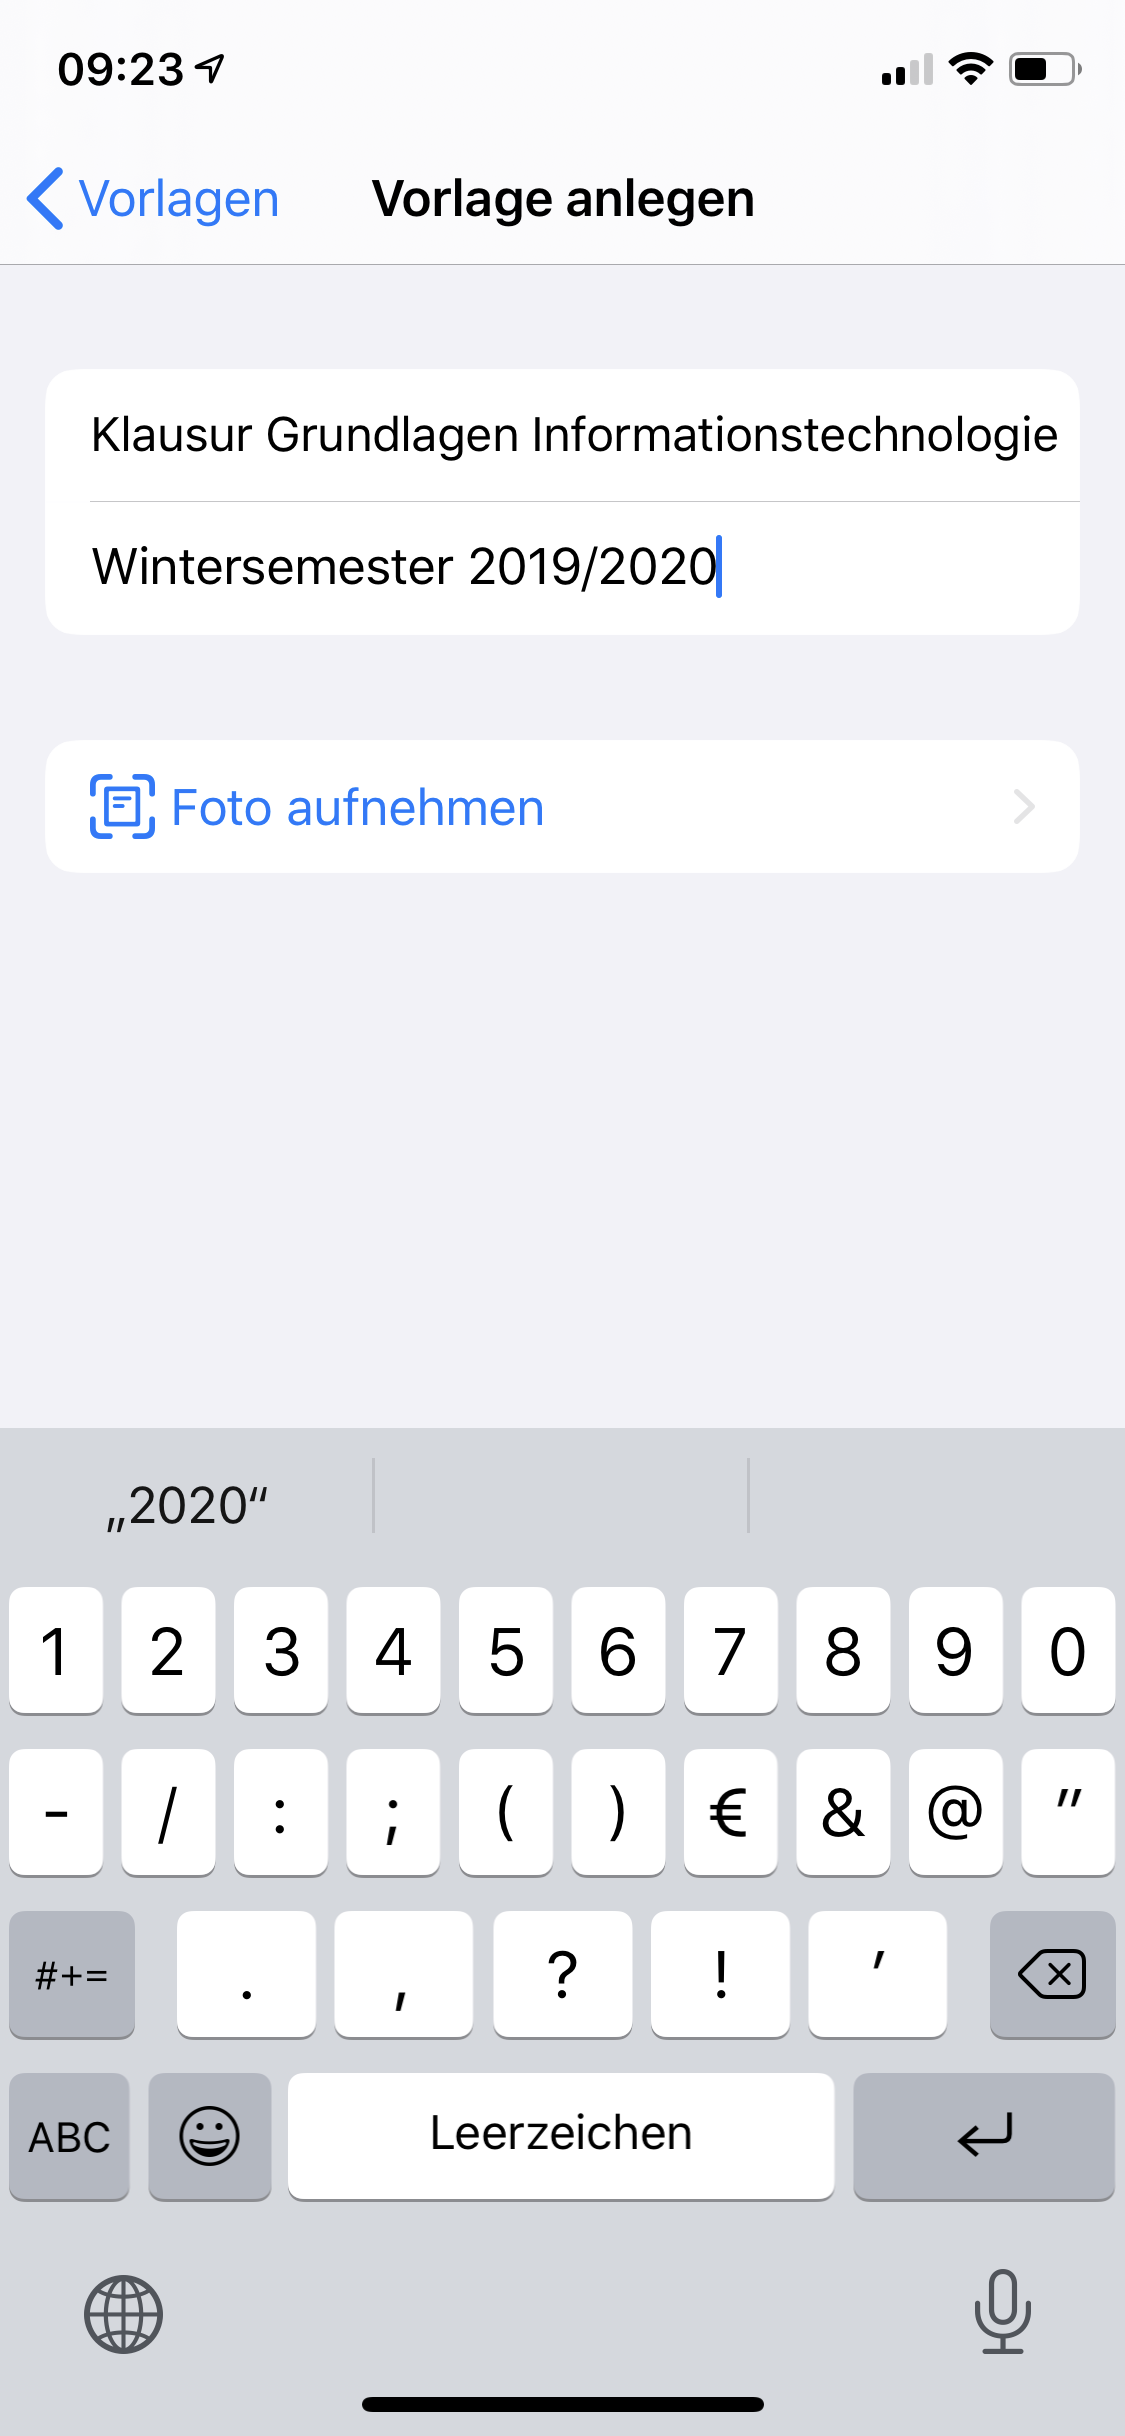
\includegraphics[width=0.96\textwidth]{img/V2}}
        			\caption{View zum Anlegen einer Vorlage}
        			\label{fig:v2}
    			\end{subfigure}
    			\begin{subfigure}[t]{0.3\textwidth}
        			\frame{\includegraphics[width=0.96\textwidth]{img/V3}}
        			\caption{Kamera- Scan-View mit Dokumenten-Erkennung}
        			\label{fig:v3}
    			\end{subfigure}
    			\begin{subfigure}[t]{0.3\textwidth}
       				\frame{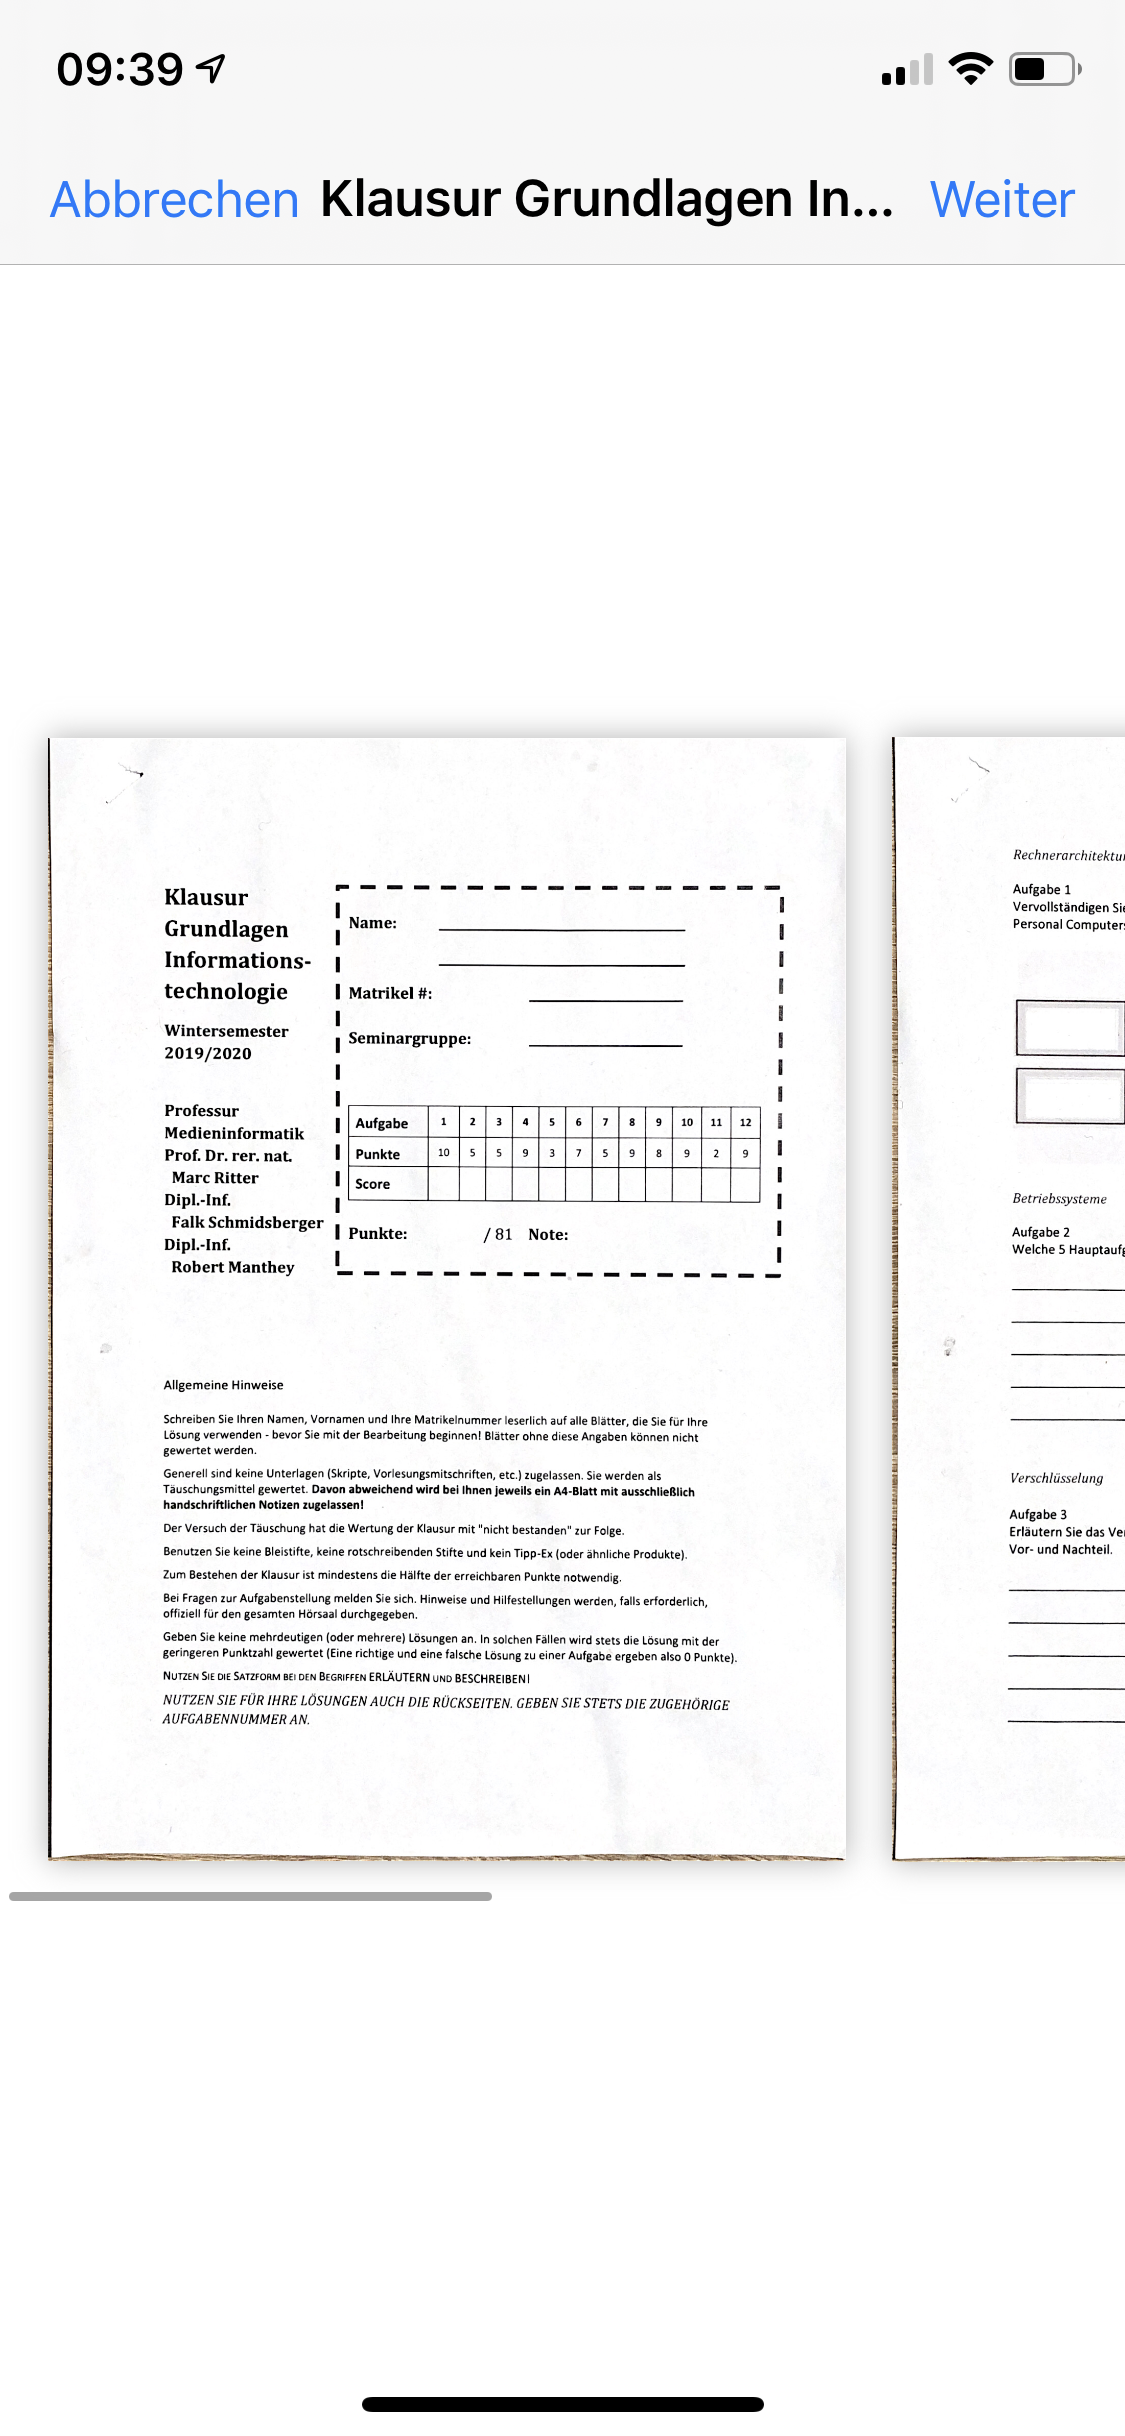
\includegraphics[width=0.96\textwidth]{img/V4}}
        			\caption{Seiten-Auswahl-View}
        			\label{fig:v4}
    			\end{subfigure}
    			\caption{Die ersten Views zur Erstellung einer Scan-Vorlage}\label{fig:erstellung1}
			\end{figure}
			Im ersten Schritt sind ein Name und weitere Informationen, zu der Vorlage an zugegeben (\ref{fig:v2}), um im Anschluss die Fotos aufzunehmen. Bei der Kamera-View (\ref{fig:v3}) handelt es sich um die Scan-View des Frameworks VisionKit. Mithilfe von Kantenerkennung und anderen Algorithmen, die Tobias Kallauke in seinem Bericht beschreibt, kann dass Dokument sobald es erkannt ist, automatisch fotografiert werden. In Echtzeit wird das erkannte Dokument aus dem Bild ausgeschnitten und gerade gezogen. Ein manuelles Auslösen des Fotos und Anpassen der Dokumenten-Kanten im Bild, ist ebenfalls möglich. Des Weiterem werden alle erstellten Bilder zu einer Gruppe gesammelt. Diese können vor dem Abspeichern angeschaut und nochmal bearbeitet werden. 
			
			\subsubsection{Regionen erstellen}
			\begin{figure}[th]
    			\centering
    			\begin{subfigure}[t]{0.3\textwidth}
        			\frame{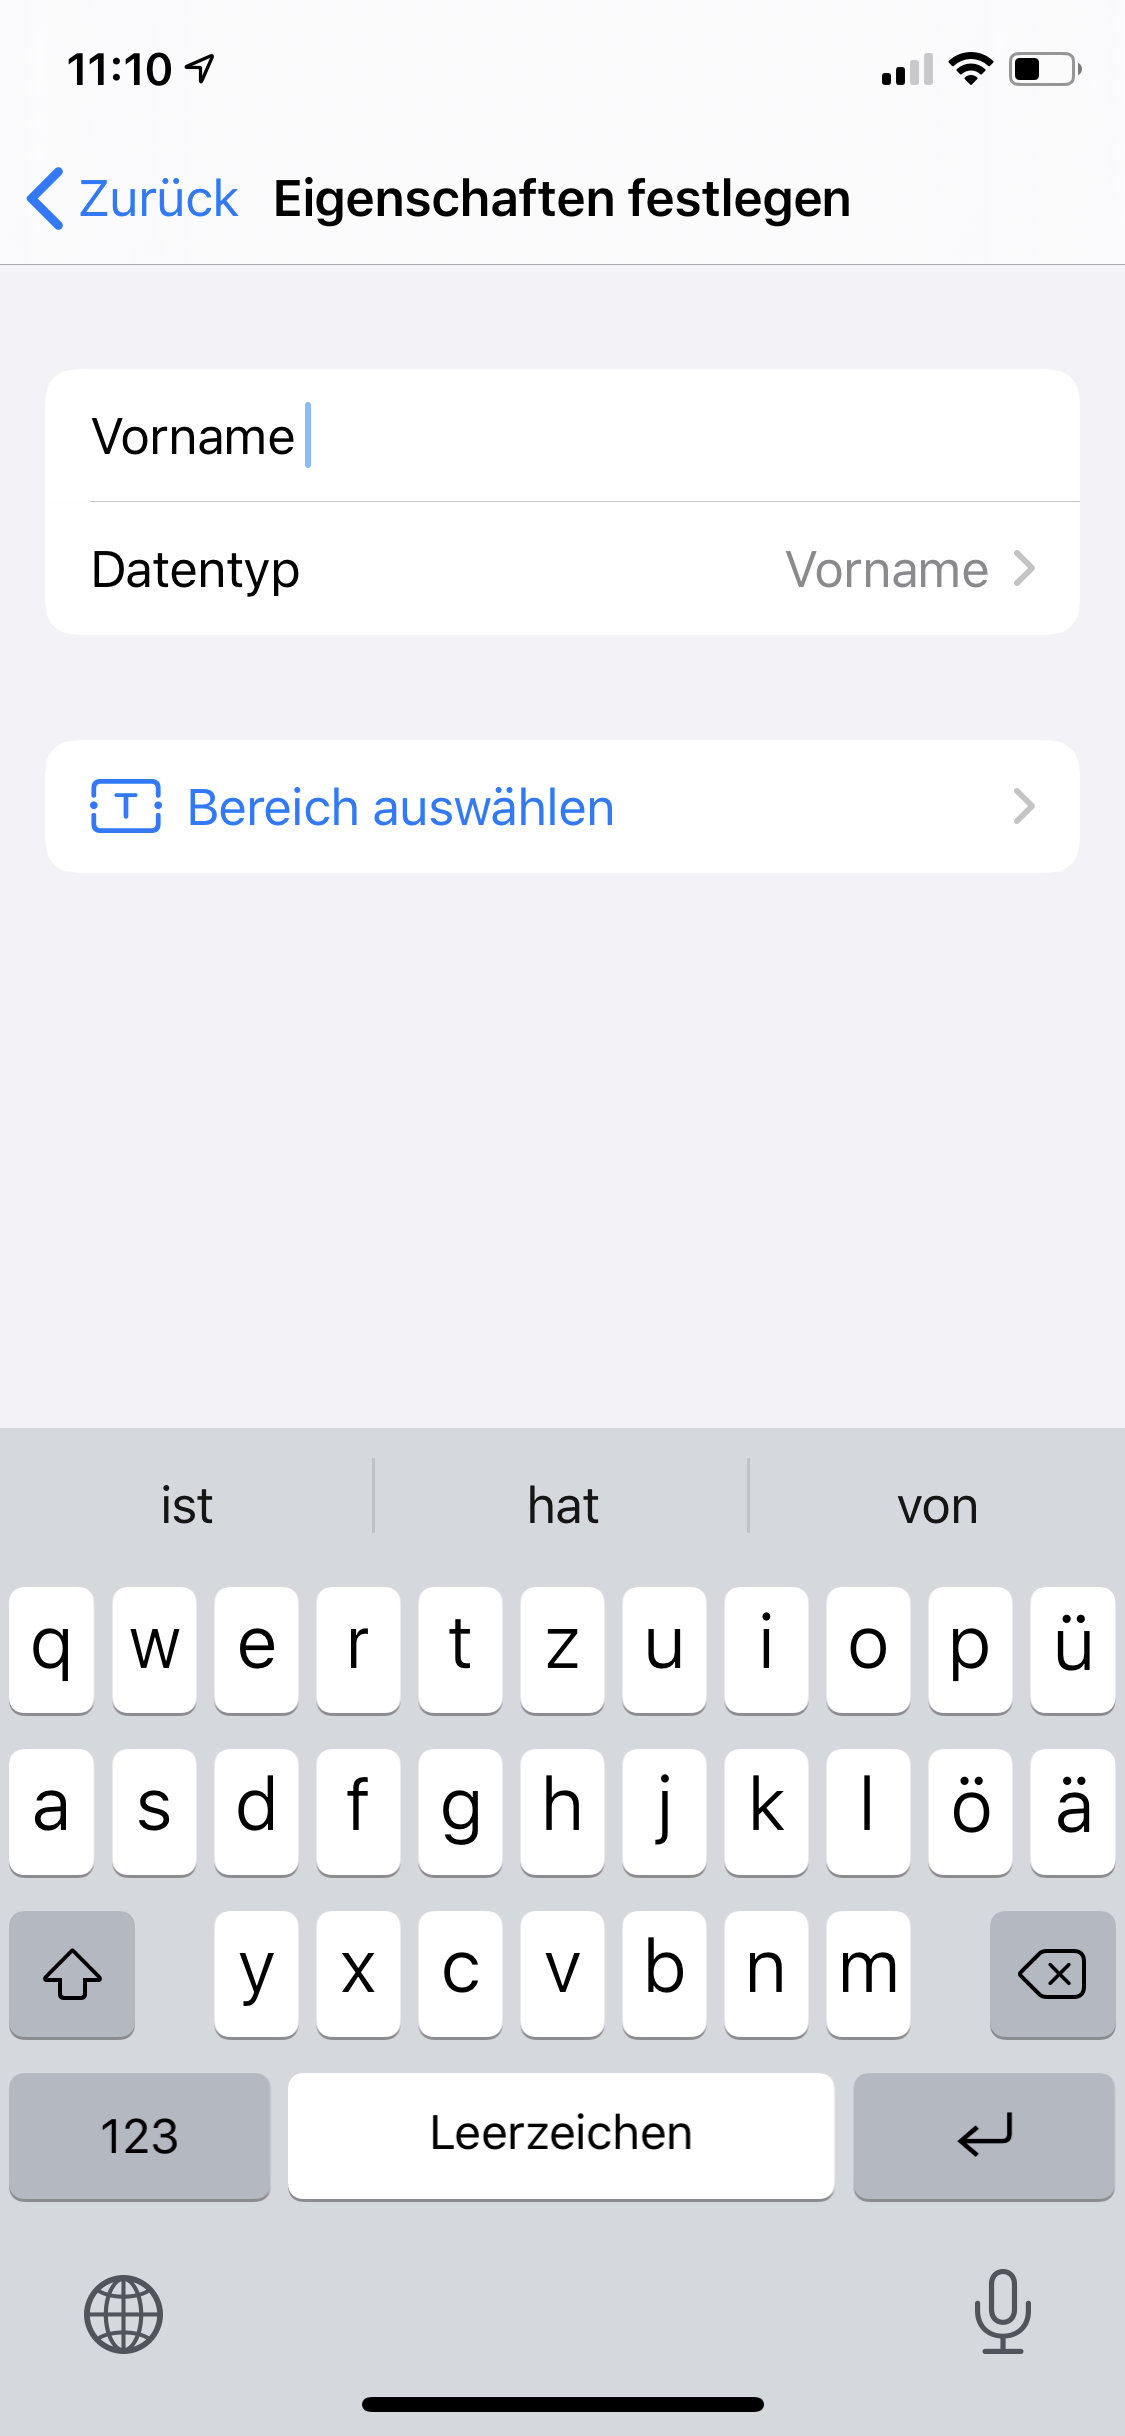
\includegraphics[width=0.96\textwidth]{img/V5}}
        			\caption{View zum Festlegen von den Regionen Eigenschaften}
        			\label{fig:v5}
    			\end{subfigure}
    			\begin{subfigure}[t]{0.3\textwidth}
        			\frame{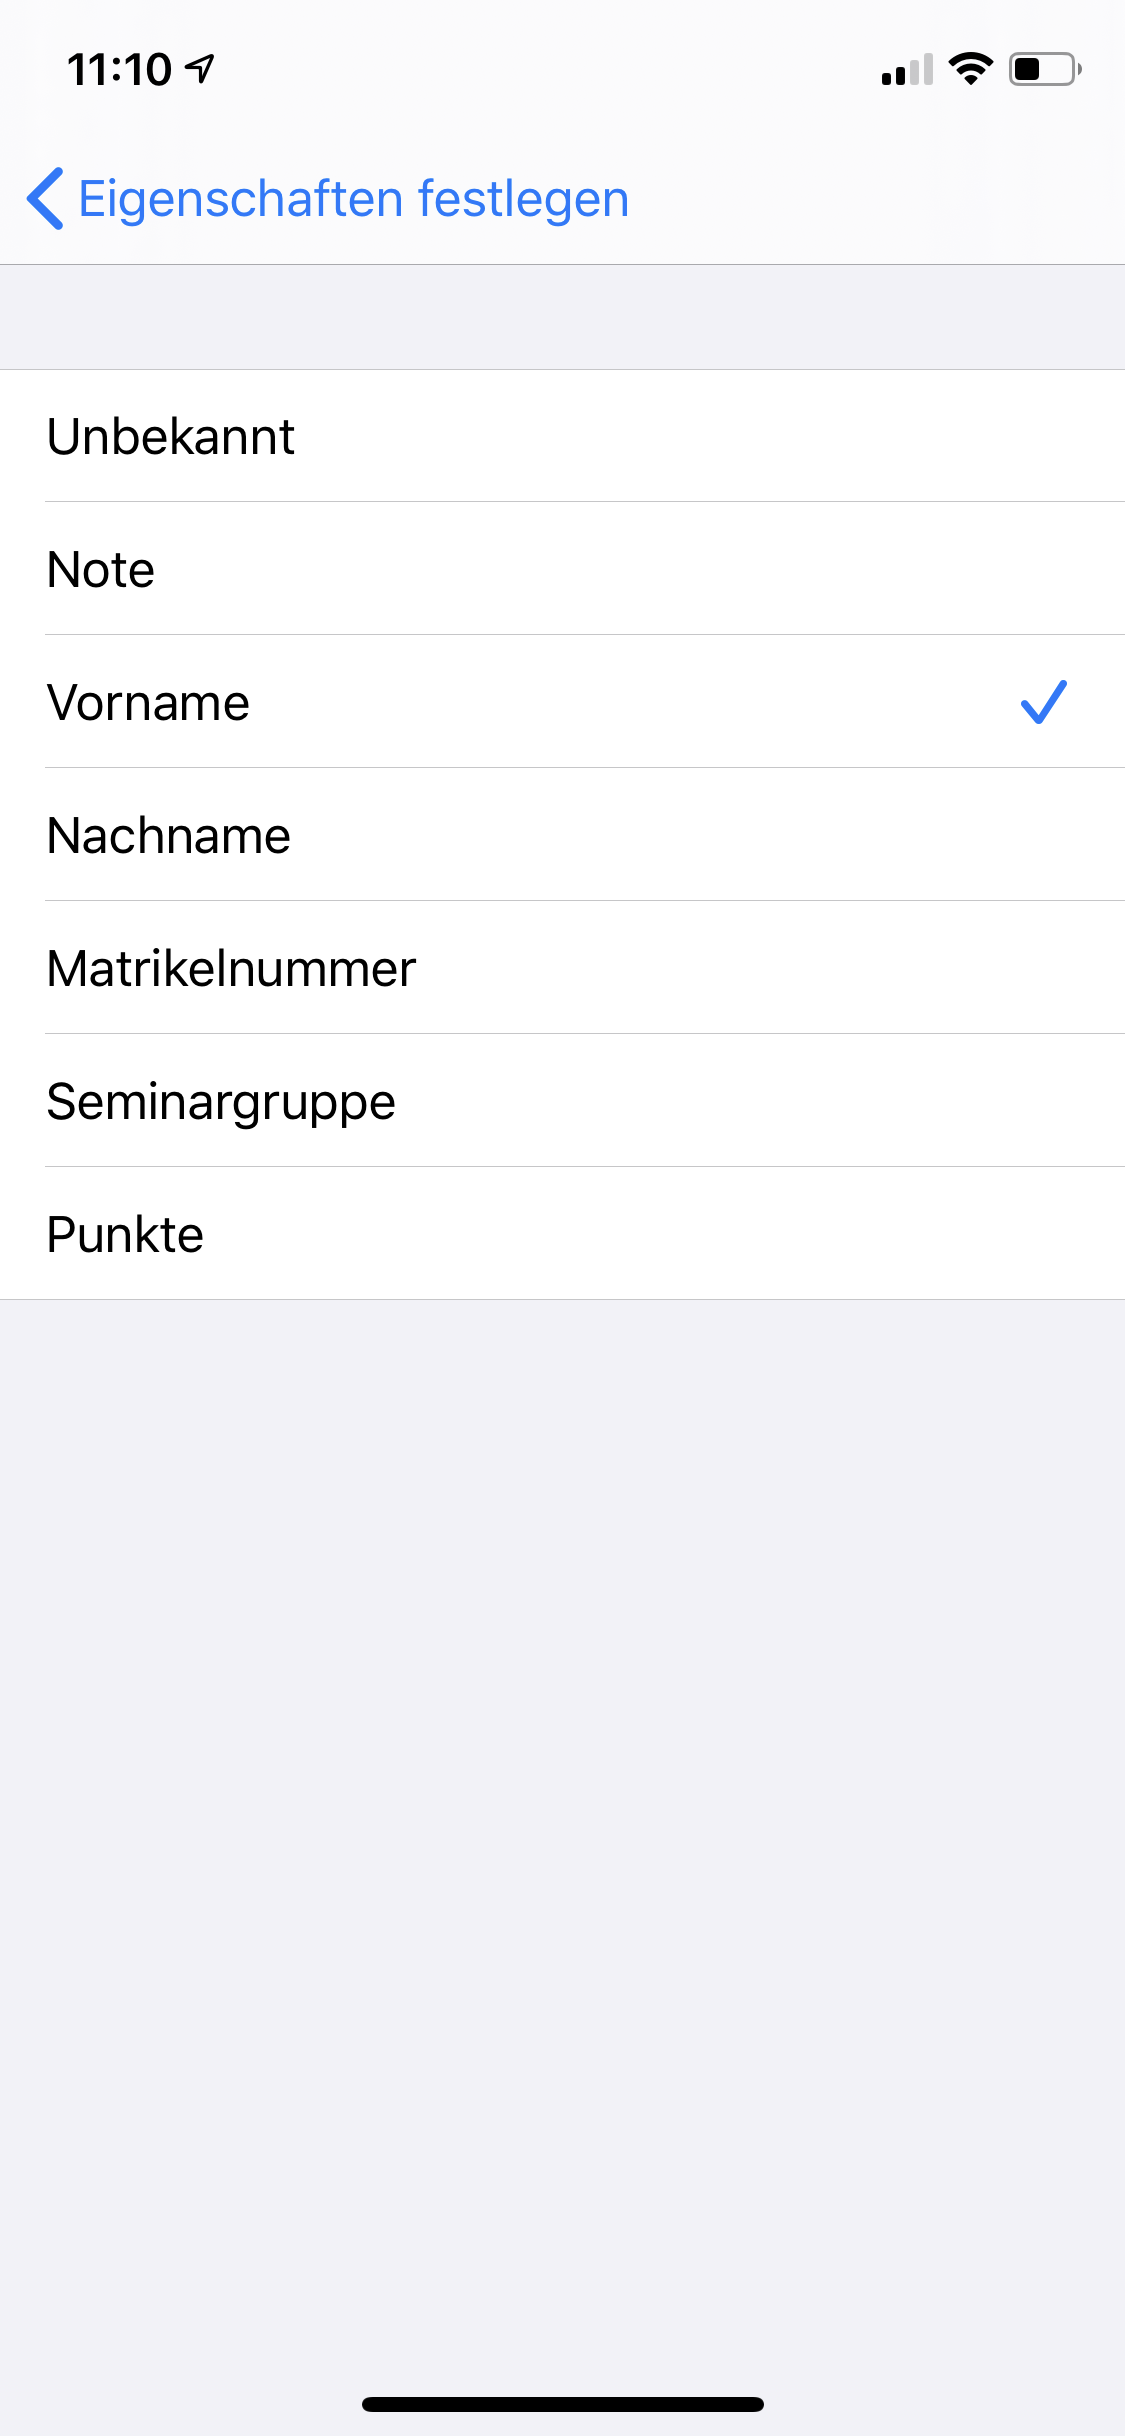
\includegraphics[width=0.96\textwidth]{img/V6}}
        			\caption{Auswahl des Datentyps}
        			\label{fig:v6}
    			\end{subfigure}
    			\begin{subfigure}[t]{0.3\textwidth}
       				\frame{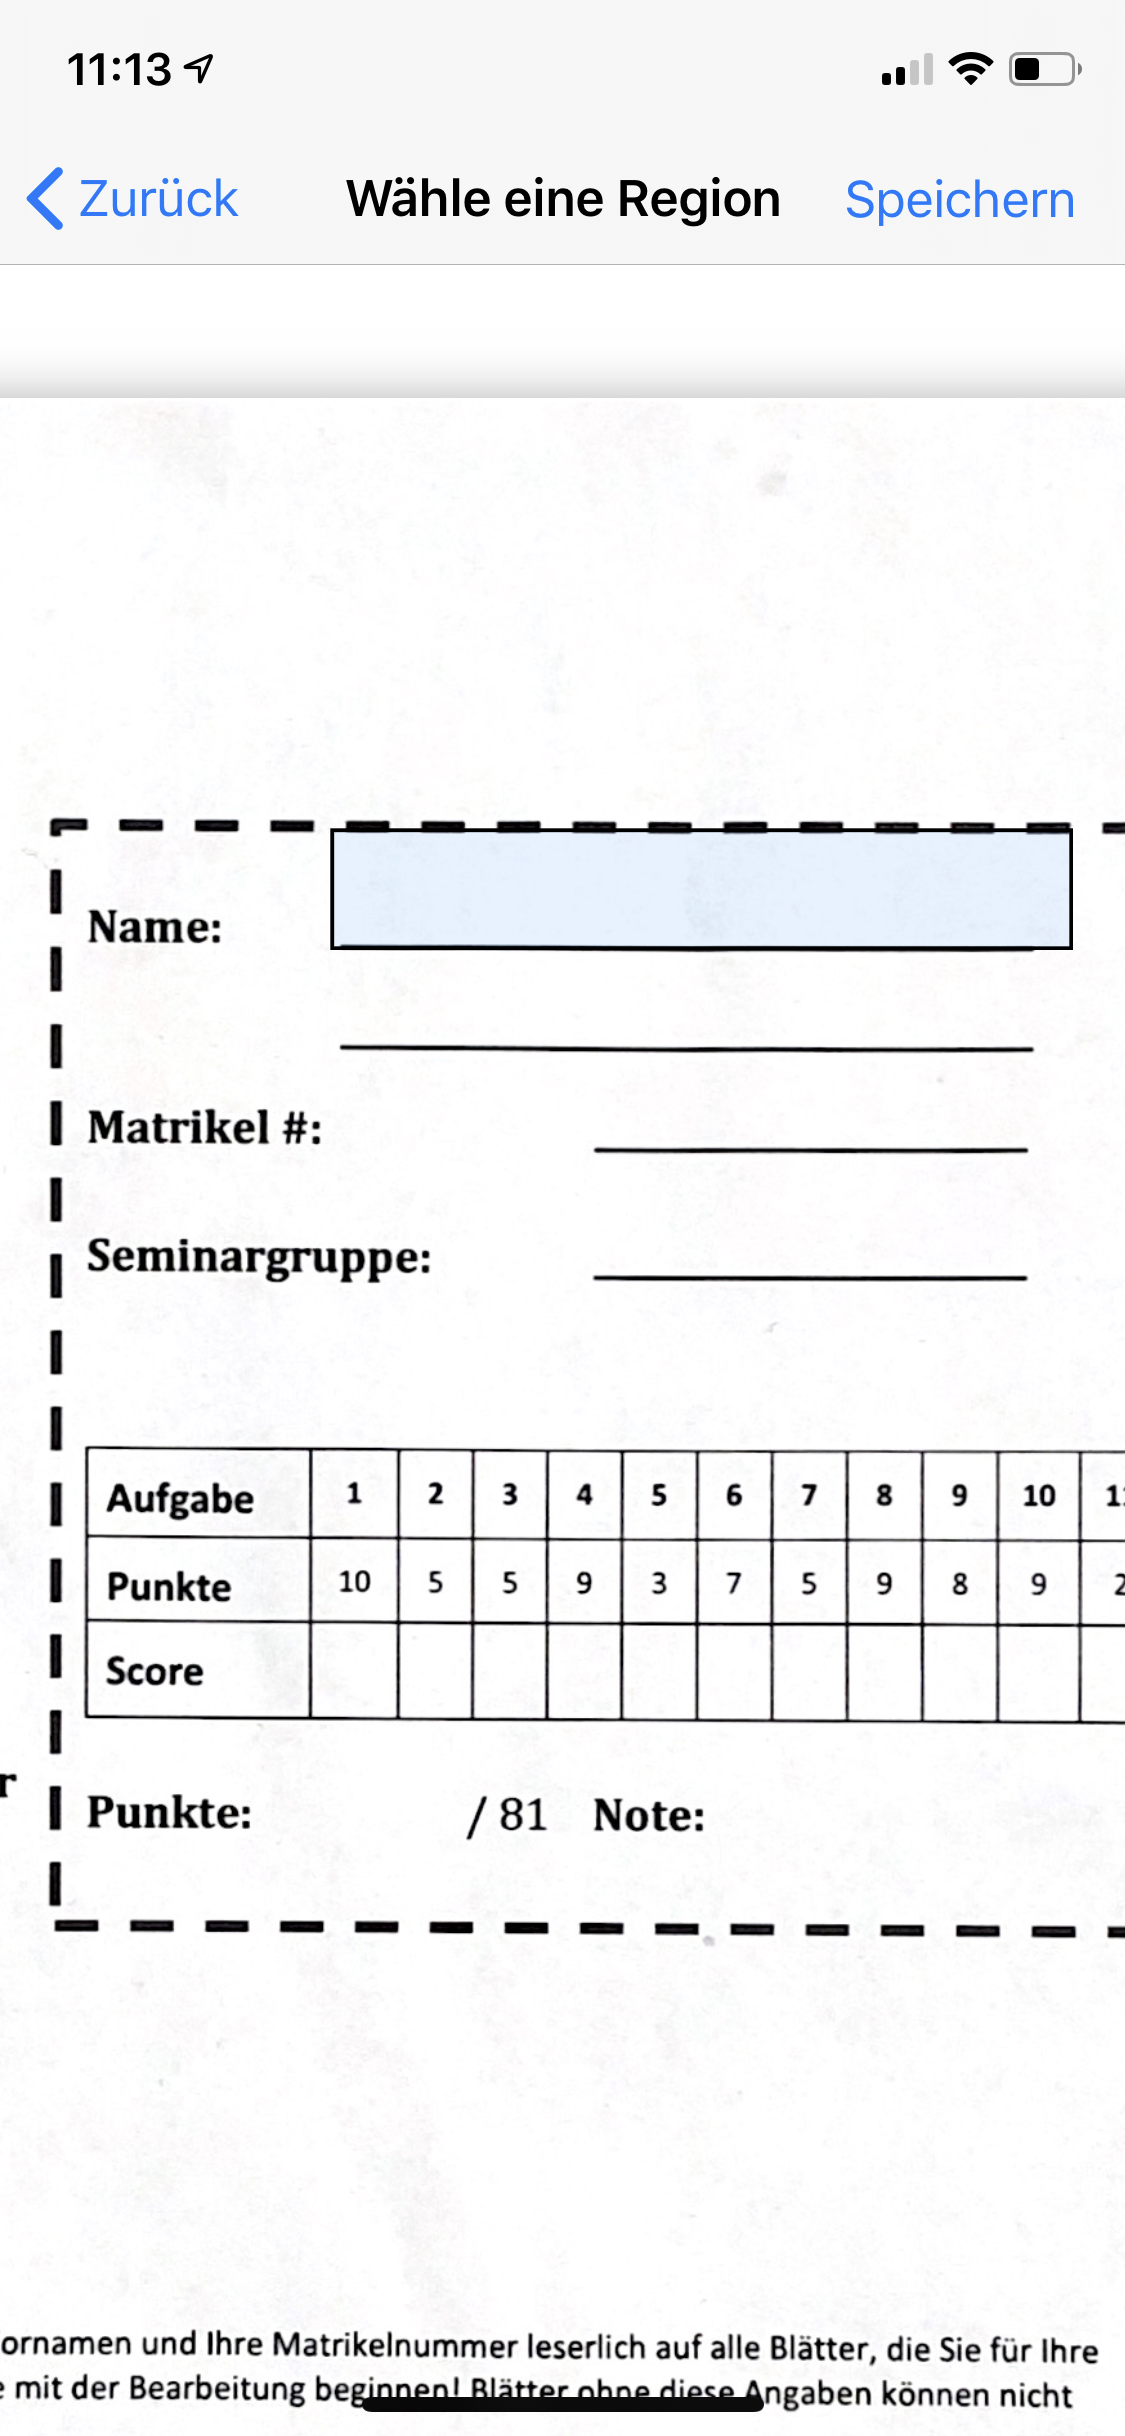
\includegraphics[width=0.96\textwidth]{img/V7}}
        			\caption{Markierung der Region auf dem Dokument}
        			\label{fig:v7}
    			\end{subfigure}
    			\caption{Views zur Erstellung von Regionen}
    			\label{fig:erstellung2}
			\end{figure}
			Im nächsten Schritt sind die Regionen auf den Dokumenten-Seiten zu markieren, deren Inhalt beim Einscannen digitalisiert werden soll. Zu erst wird die gewünschte Seite aus einer Übersicht (\ref{fig:v4}) ausgewählt. Anschließend ist eine Vorschau der Seite mit alle eingetragenen Regionen zu sehen (\ref{fig:v8} bzw. \ref{fig:v9}). Über einen Button können weitere Regionen hinzugefügt werden. Dazu legt man einen Namen (\ref{fig:v5}) und einen Datentyp (\ref{fig:v6}) fest. Die Datentypen sind für die Texterkennung und für die Erstellung der Tabelle für die Notenfreigabe wichtig. Dazu später mehr. Wenn die Eigenschaften der Region festgelegt sind, muss diese noch auf dem Bild markiert werden. Dazu zieht man mit einem Finger ein Rechteck in einer beliebigen Größe ein (\ref{fig:v7}). Die markierte Region kann anschließend noch bewegt oder neu gemacht werden. Um kleinere Regionen präzise zu markieren kann mit einer Zwei-Finger-Geste auch an die Seite heran bzw. auch heraus gezoomt werden. Dieses Vorgehen muss dann für alle nötigen Regionen auf den jeweiligen Seiten wiederholt werden. 
			\begin{figure}[th]
    			\centering
				\begin{subfigure}[t]{0.3\textwidth}
       				\frame{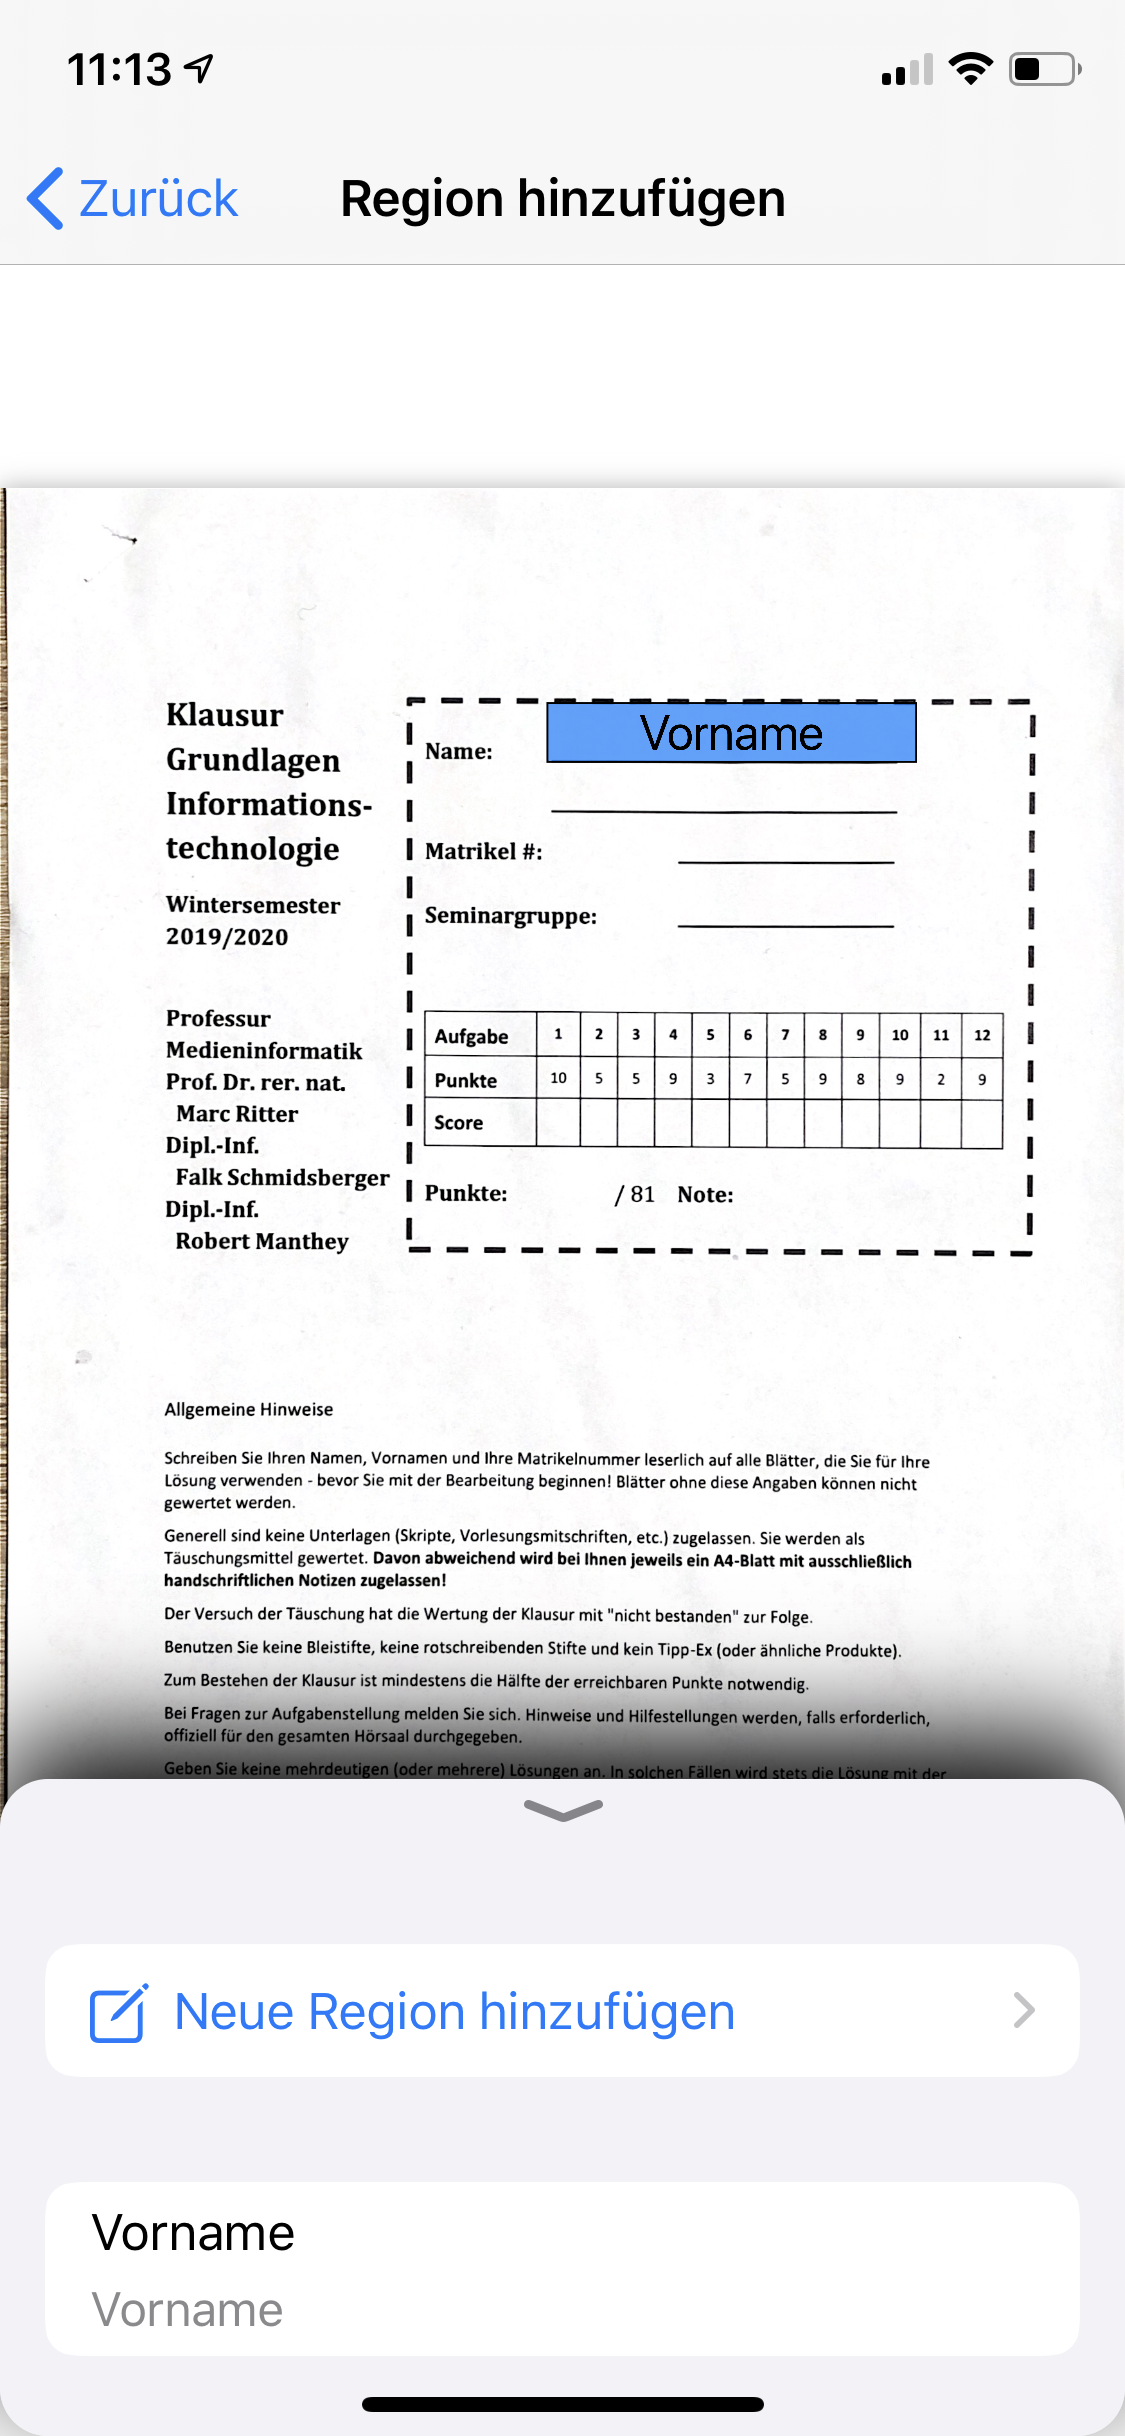
\includegraphics[width=0.96\textwidth]{img/V8}}
        			\caption{Seiten-Vorschau mit der ersten Region}
        			\label{fig:v8}
    			\end{subfigure}
    			\begin{subfigure}[t]{0.3\textwidth}
       				\frame{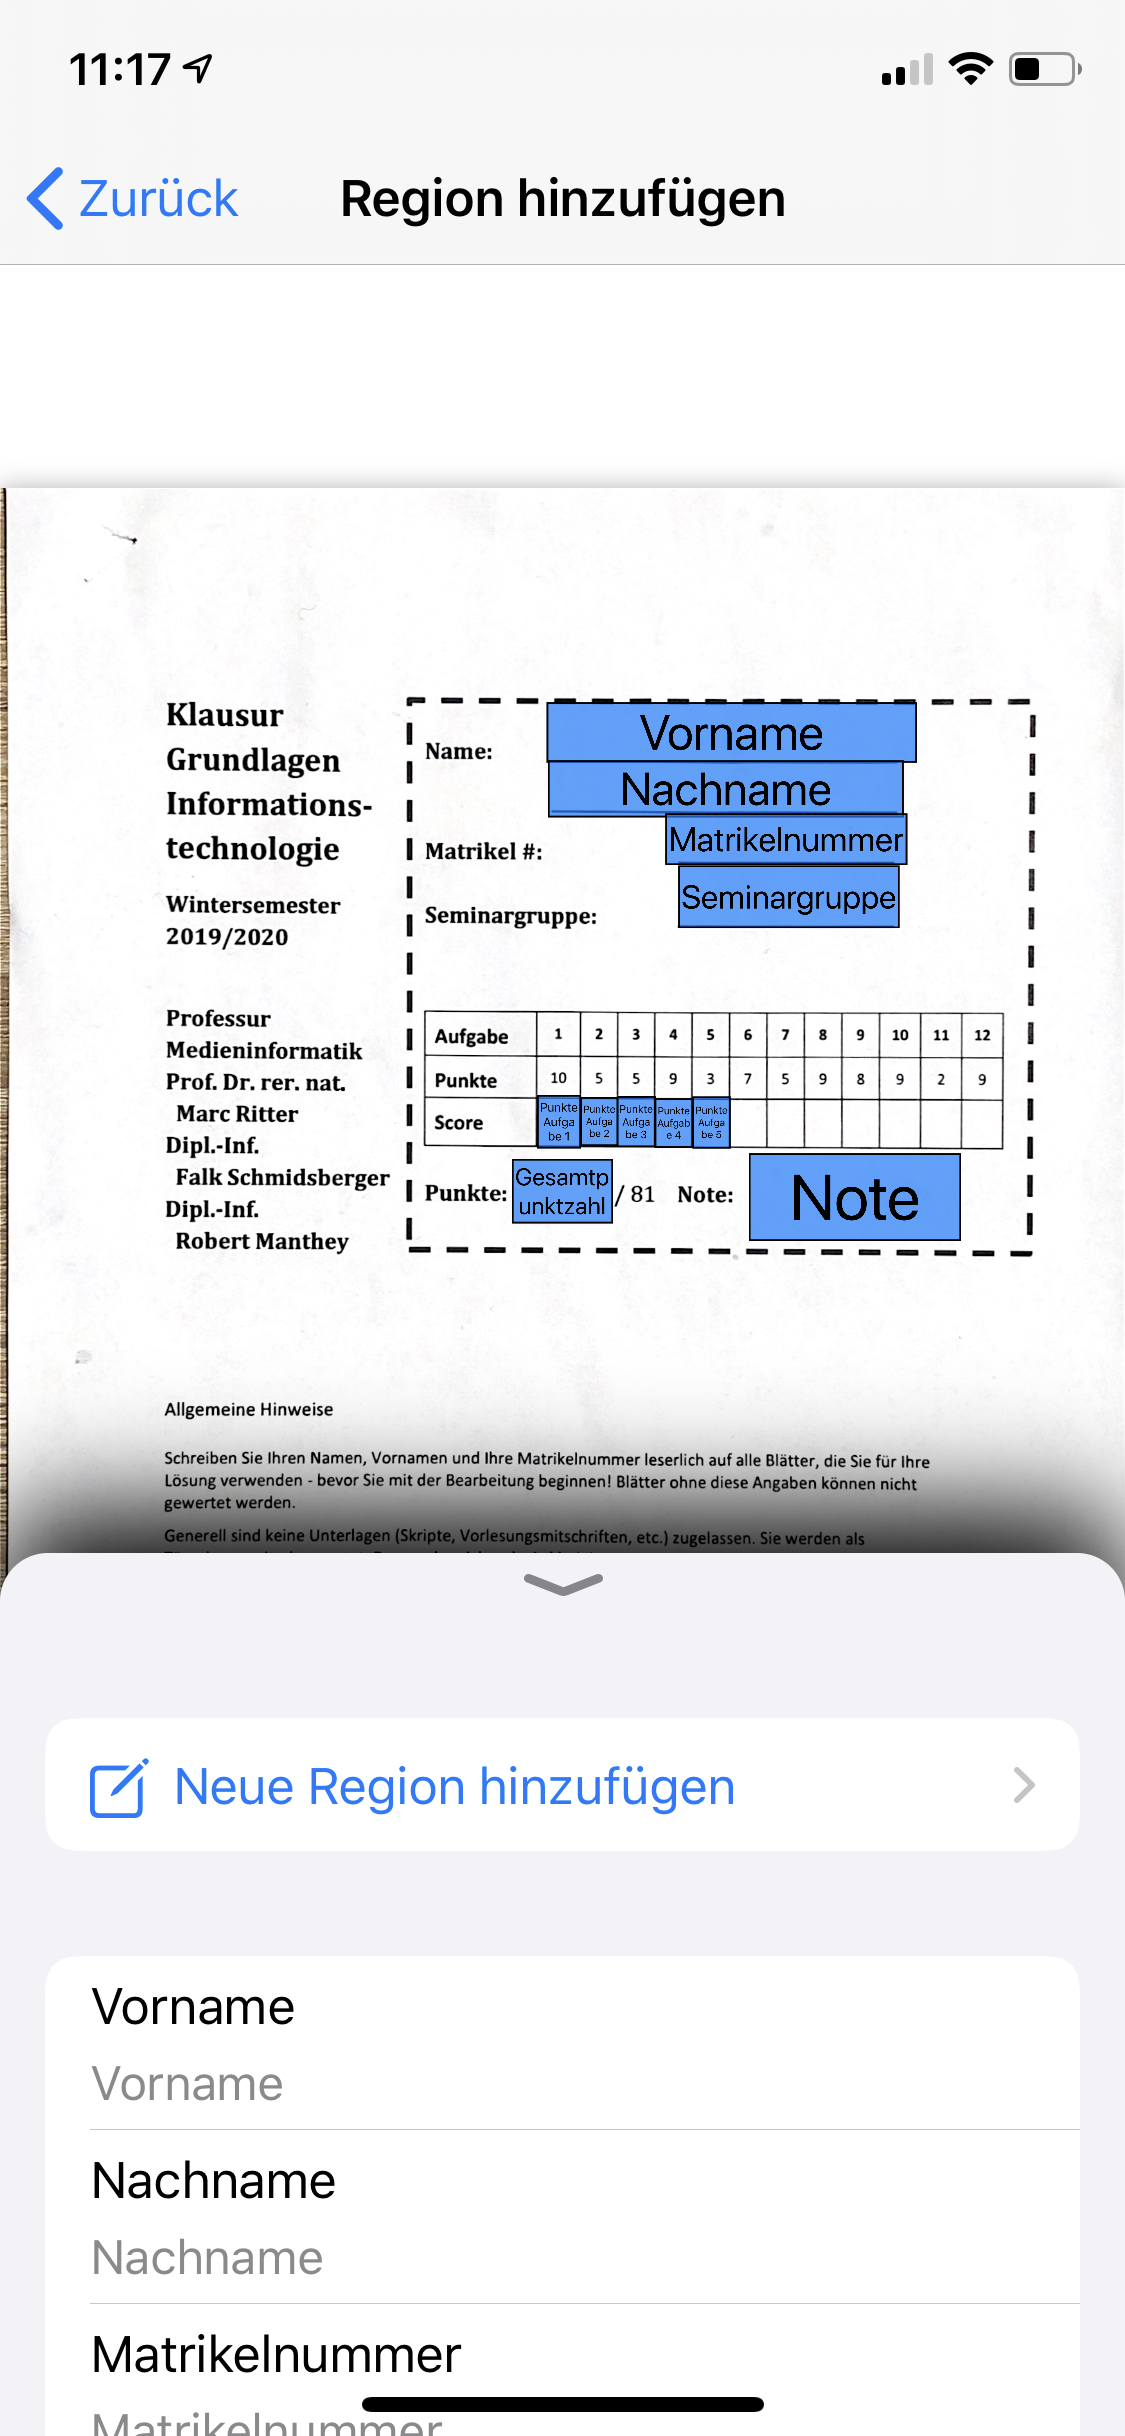
\includegraphics[width=0.96\textwidth]{img/V9}}
        			\caption{Seiten-Vorschau mit allen Regionen}
        			\label{fig:v9}
    			\end{subfigure}
    			\begin{subfigure}[t]{0.3\textwidth}
       				\frame{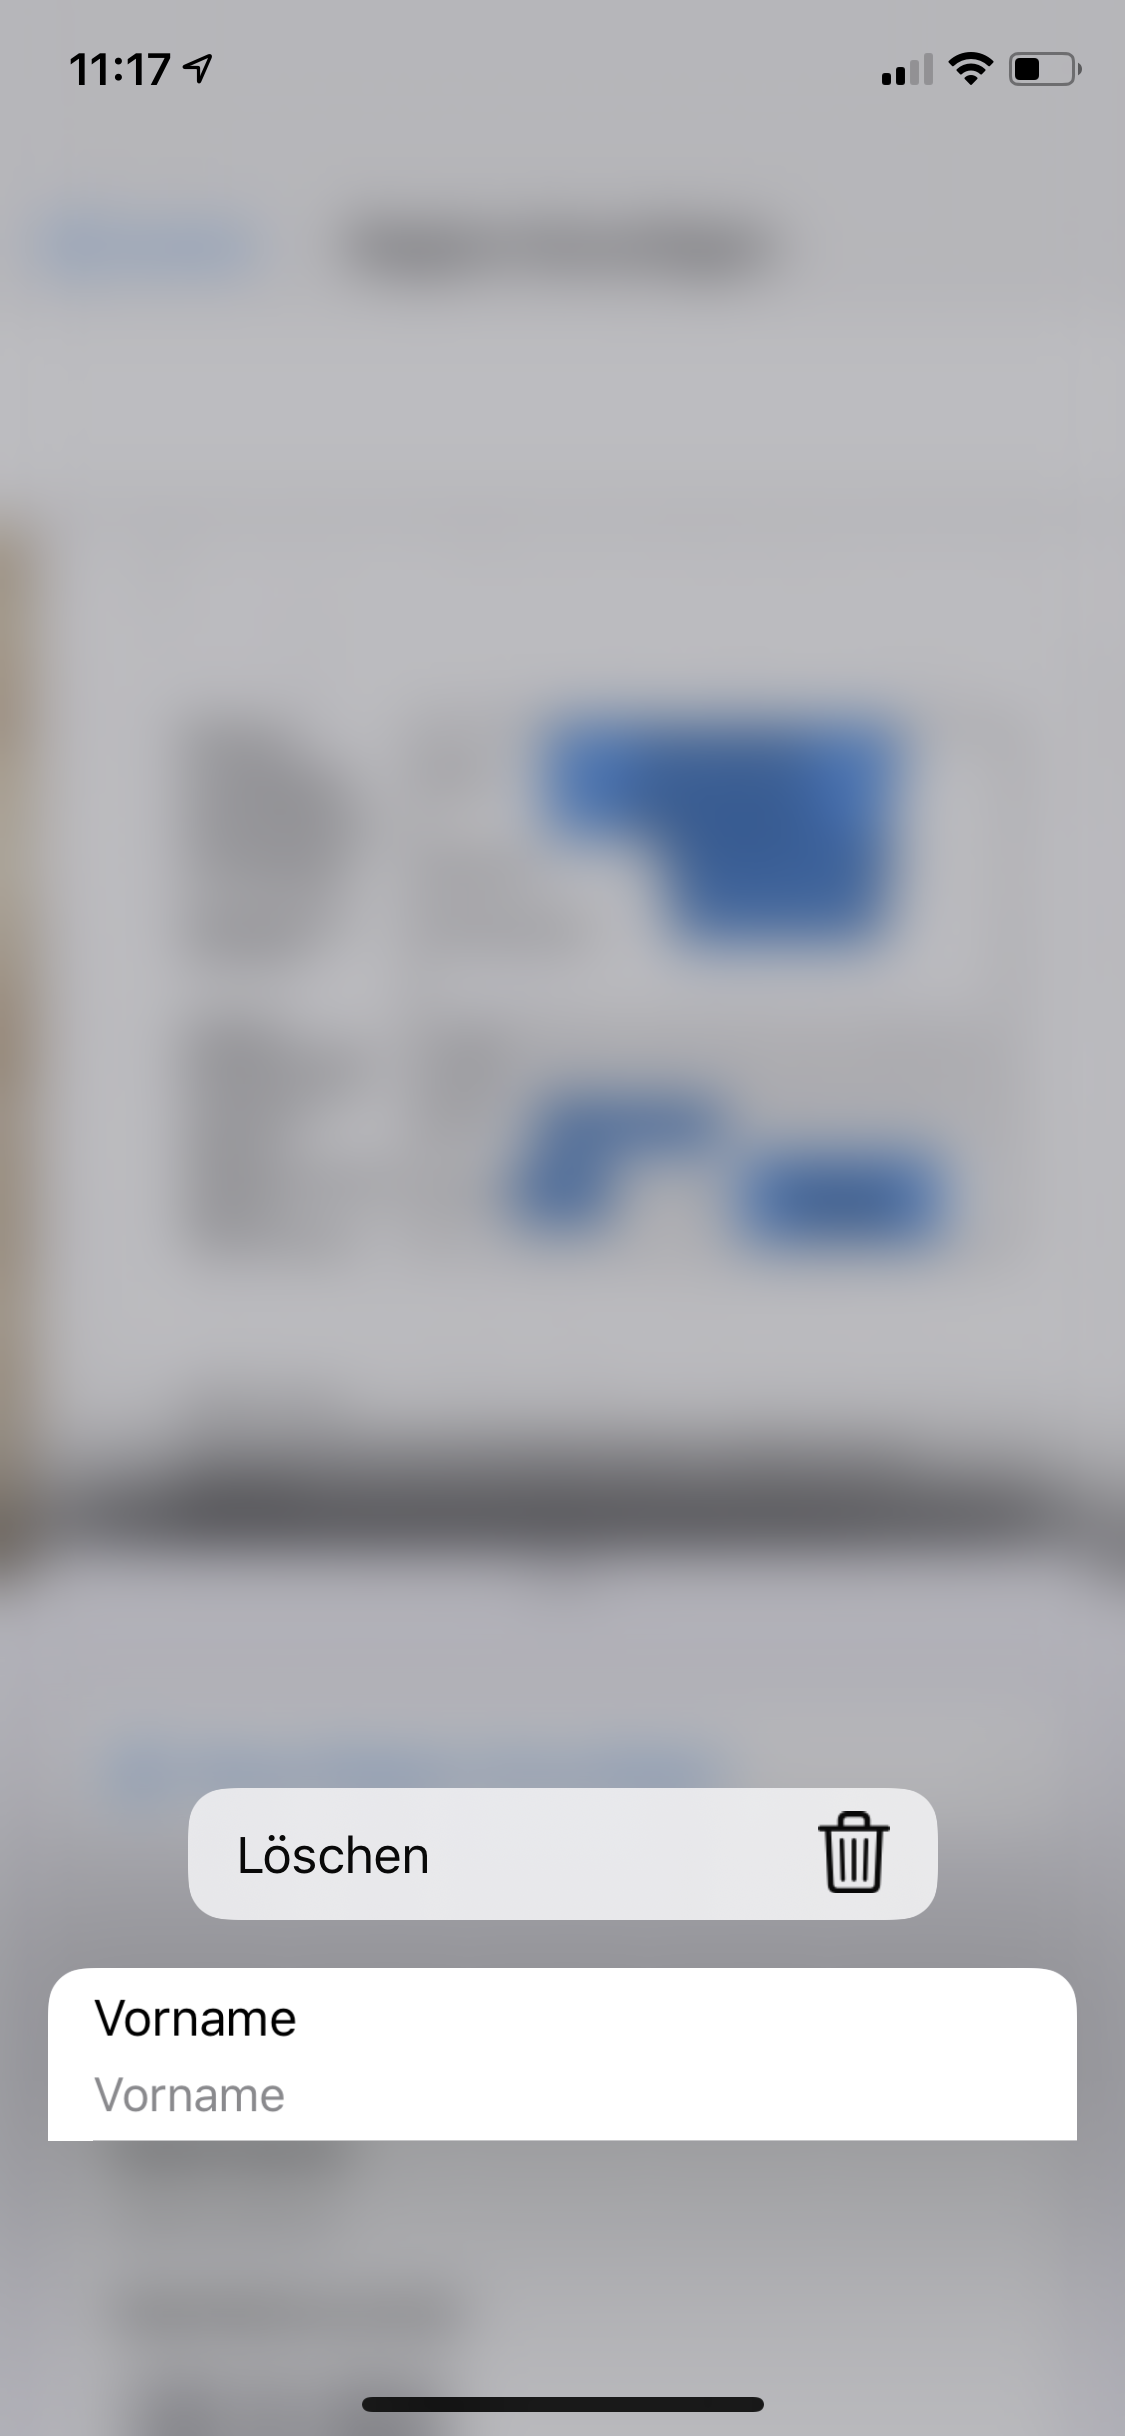
\includegraphics[width=0.96\textwidth]{img/V10}}
        			\caption{Löschen einer angelegten Region}
        			\label{fig:v10}
    			\end{subfigure}
    			\caption{Seiten-Vorschau-View}
				\label{fig:erstellung3}
			\end{figure}
			
			\subsubsection{Links erstellen}
			Zum Schluss können noch die sogenannte Links erstellt werden. Diese Funktion ist allerdings noch nicht sehr weit fortgeschritten und beinhaltet aktuell nur den Link-Typ zum Vergleichen von Regionen, wie im Kapitel \ref{ch:konzept} Konzept beschrieben ist. Beim Erstellen eines Vergleich-Links wählt man zwei Regionen aus, deren Inhalt nach der Texterkennung auf Gleichheit überprüft wird. 
			
			\begin{figure}[th]
    			\centering
				\begin{subfigure}[t]{0.3\textwidth}
       				\frame{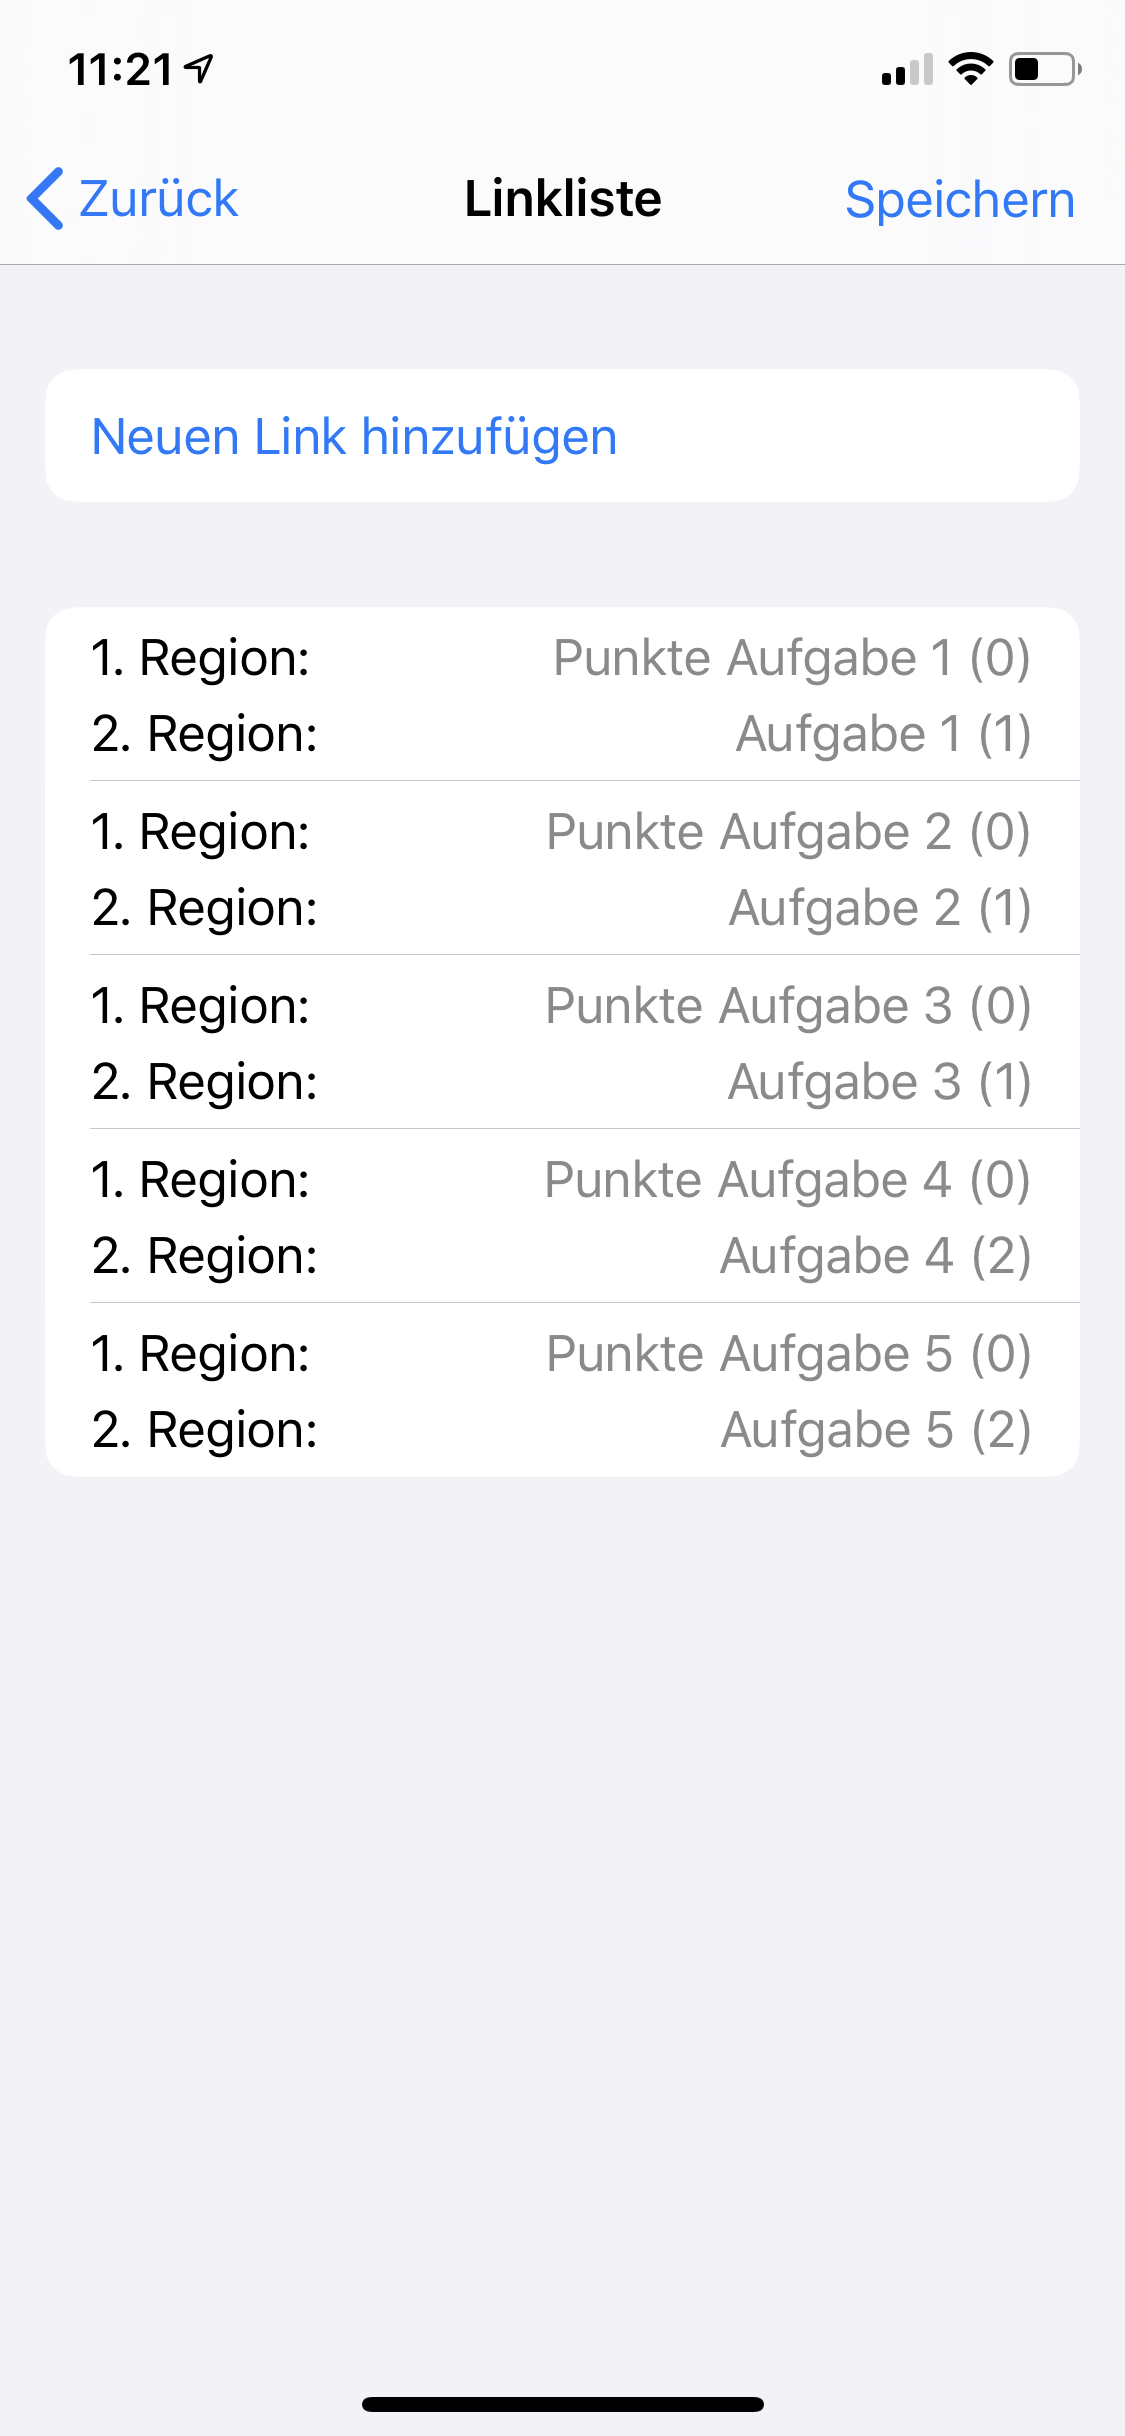
\includegraphics[width=0.96\textwidth]{img/L6}}
        			\caption{Linkliste mit angelegten Links}
        			\label{fig:l1}
    			\end{subfigure}
    			\begin{subfigure}[t]{0.3\textwidth}
       				\frame{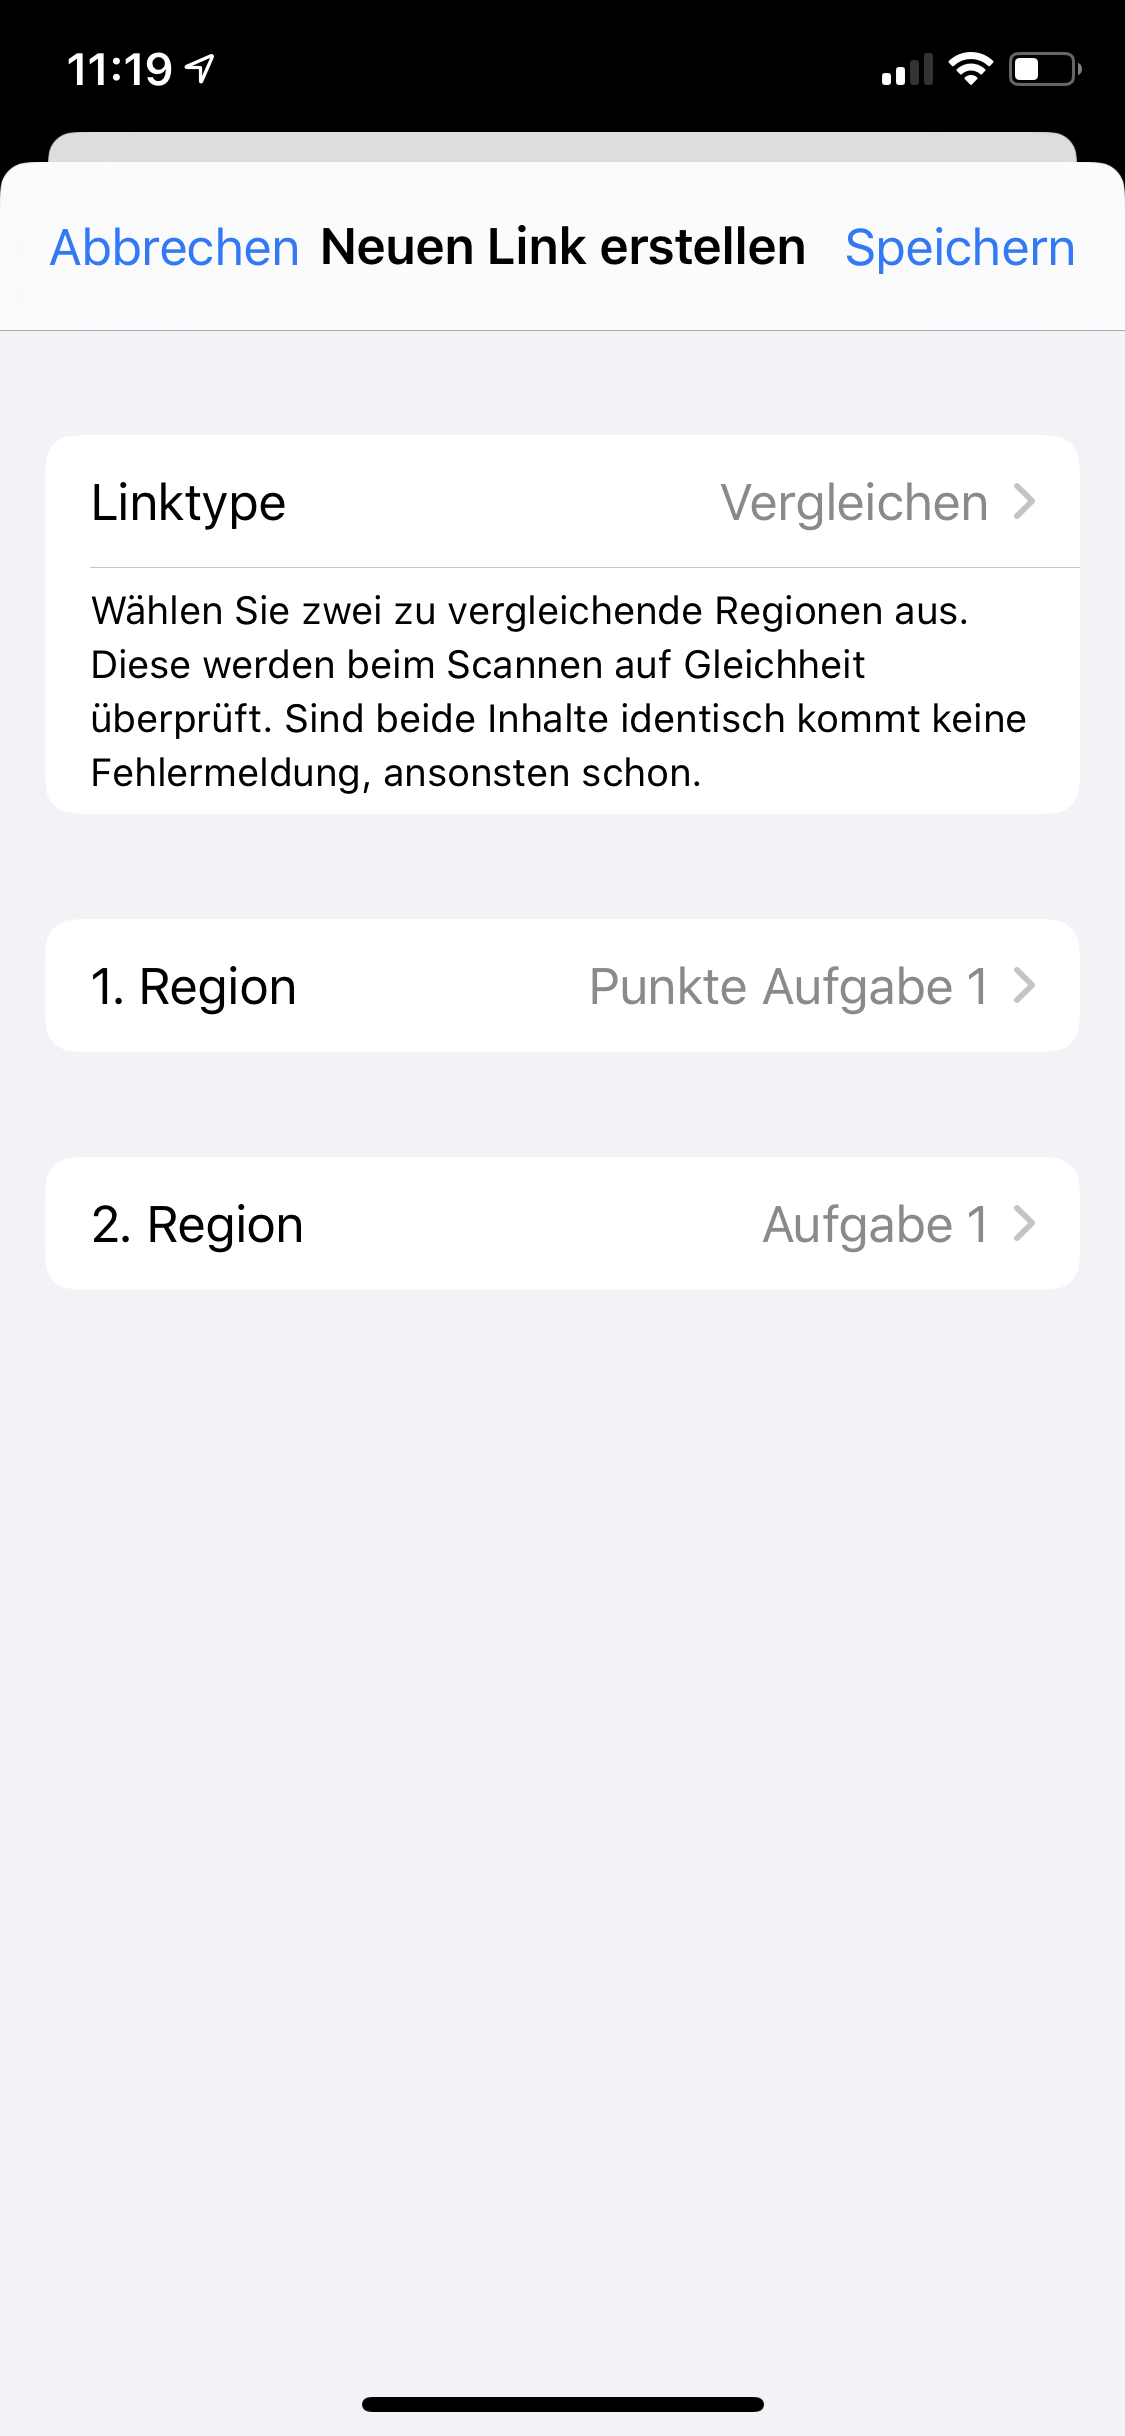
\includegraphics[width=0.96\textwidth]{img/L4}}
        			\caption{View zur Erstellung eines Vergleich-Links}
        			\label{fig:l2}
    			\end{subfigure}
    			\begin{subfigure}[t]{0.3\textwidth}
       				\frame{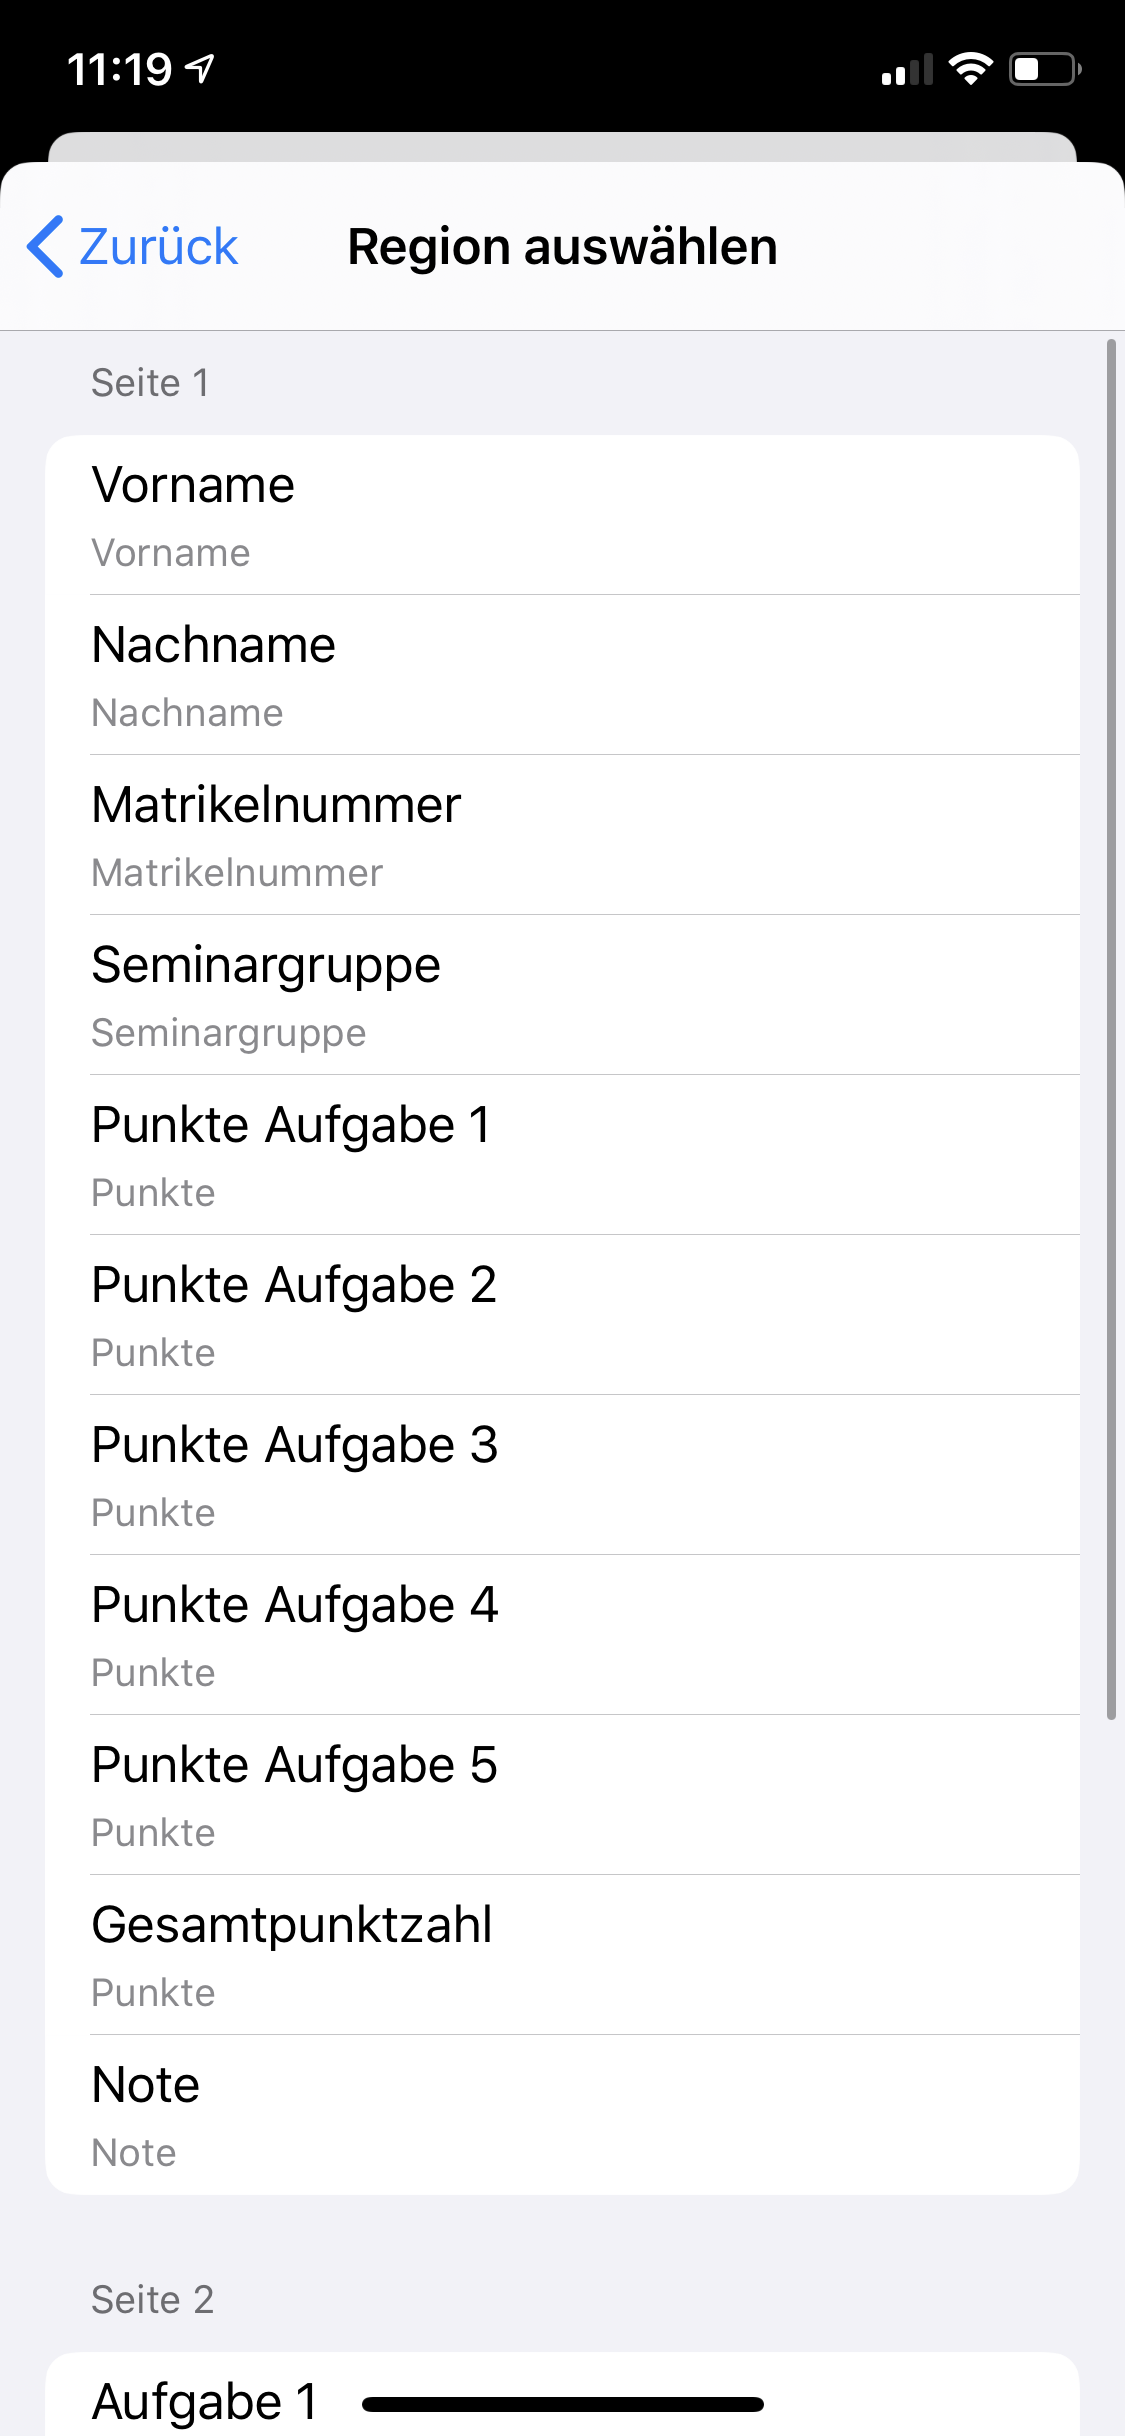
\includegraphics[width=0.96\textwidth]{img/L3}}
        			\caption{View zur Auswahl einer Region}
        			\label{fig:l3}
    			\end{subfigure}
    			\caption{Seiten-Vorschau-View}
				\label{fig:link1}
			\end{figure}
		
			\subsubsection{Vorlage speichern}
			Wenn eine Vorlage gespeichert werden soll, passiert das in mehreren Schritten. 
			\begin{enumerate}
				\item Der Name und die Beschreibung der Vorlage sowie die Liste an Links wird gesendet. In der Antwort des Servers befindet sich dann die Vorlagen-ID, die in den nächsten Schritten benötigt wird. 
				\item Die Bilder der Seiten werden gesendet. Als Antwort zu jedem Bild wird der Pfad geschickt, wo das Bild gespeichert wurde. Dieser Pfad wird im nächsten Schritt benötigt.
				\item Die Seiten mit einer Seiten Nummer und dem Pfad zu dem Bild, wird mit der Vorlagen-ID gesendet. Als Antwort wird eine ID zurückgegeben, die im nächsten Schritt verwendet wird.
				\item Die Regionen der Seiten werden gesendet. Eine Region, auch Attribut genannt hat X- und Y-Koordinaten. Diese repräsentieren den Abstand vom Bildursprung, der sich in jedem Bild oben links befindet. Außerdem besitzt eine Attribut eine Höhe und Breite, einen Namen und einen Datentyp. Zusammen mit der Seiten-ID wird das Attribute an den Server gesendet.
			\end{enumerate}
		
		\subsection{Vorlage verwenden}
		

		
		- keine Unit Tests etc. keine Zeit
		
	\section{''Abnahme''}	
		Abnahme ... 
		
	- Accessibility 	von Haus aus etwas... dank swiftui
	- wie benutze ich die App wie installiere ich die
	- 
		\\ \\ \\
	Weitere Punkte die in Kapitel 6 rein könnten/sollten: 
	
	- beschreiben wie die einzelnen Views/Seiten nun aussehen und funktionieren? oder eher den Prozess der Entwicklung?
	
	- Bild mit Wireframe aller Views und deren Workflow?
	
	- erklären deskew / Dokument ausrichten?
	
	- Umrechnung der Bilder vom Template aus und zuschneiden der neuen Regionen erklären
	
	- Attribute hinzufügen (den Vorgang) -> Rechteck einzeichnen...
	
	- Verwendete Programme, Sprache, etc. 
	
	- ein paar Worte, wie gut die Entwicklung lief (Simulator vs. echtes Gerät), wo sind die Grenzen des Simulators (Keine Kamera), wo waren Probleme mit dem echten Gerät...

%%%%%%%%%%%%%%% - WEITERENTWICKLUNG - %%%%%%%%%%%%%%%

\chapter{Weitere Entwicklung und Besonderheiten}
	
	\section{API}
		- auf die API eingehen? oder nur Tobias?
	
	\section{}
		- Keyboards
		- Accsessebility
		
%%%%%%%%%%%%%%% - GRENZEN - %%%%%%%%%%%%%%%

\chapter{Grenzen der App}
	\section{Probleme beim Erkennen von Dokumenten}
		- Gleich-farbiger Hintergrund
			
		- Wenig Licht
		
		- Hintergrund mit starken Kanten
		
		- Runde Ecken, keine Ecken
		
		- Starke Kanten im Bild (schwarzer Kreditkartenstreifen)
		
		- zu jedem möglichem vlt. dann ein Beispiel Bild
		
	\section{Probleme der Klausur-Vorlage beim Scannen}
		- Schrift zu klein
		
		- zu wenig Platz
		
		- zu viel Platz
		
		- Überschneidungen
		
		- ...
		
	\section{Weitere ...}
		- Abstürze, Memory Leaks, 



%%%%%%%%%%%%%%% - TEMPLATES - %%%%%%%%%%%%%%%

\chapter{Templates}
	- Template und den Entwicklungsprozess vorstellen, 
	
	- wieso weshalb warum muss das nun so aussehen?
	
	- Was kann an der neuen Vorlage immer noch optimiert werden?	
	
	- Welche Probleme konnten behoben werden?
	
%%%%%%%%%%%%%%% - AUSBLICK - %%%%%%%%%%%%%%%
		
\chapter{Ausblick}
	- Es müssen nicht nur Klausuren sein, sondern alles mögliche (Krankenscheine, Urlaubsscheine, was auch immer, nur DB muss angepasst werden. (oder automatisches generieren von DB-Tabellen an Hand der Template Attribute))
	
	- Server mit Bildern als Klausuren-Einsicht nutzen -> allerdings viele Probleme (Klausuren würden kopiert werden -> Profs mehr Arbeit, keinen direkten Kontakt zum Prof wegen Fragen, Verbesserungen oder Anmerkungen, ... )
	  (warum genau, sollen die gespeichert werden? meine/unsere Idee Online Klausureneinsicht -> ins Fazit/Ausblick (hat viele ''Probleme'' ))
	
	- QR-Code-Idee um Vorlagen weg zu lassen -> Programm oder Plugin (Word/LaTeX) was die QR-Codes dann automatisch erstellt und richtig einfügt. (Wichtige Daten sind da hinterlegt, Vor- und Nachteile von QR-Codes, ...)
	
	- Ist die App nun schneller als der normale Umgang bleibt offen -> Bachelorarbeit knüpft da an...
	
	- ImageCaptureCore für macOS
	
	- neuer Workflow. Klausur hat immer Name, Matrikel Nummer, etc. (Nicht extra Regionen-Namen vergeben)
	

\Anhang

\chapter{Workflow} \label{ch:workflow}
	\section*{Vorlage erstellen}
	\begin{enumerate}
		\item ''Neue Vorlage erstellen''
		\item Foto machen
		\item Frage: Ist Foto gut? 
		\begin{enumerate}
			\item Ja: gehe zu 4.
			\item Nein: gehe zu 2.
		\end{enumerate}
		\item Neues Attribut hinzufügen
		\item Bereich auf Bild auswählen
		\item Frage: Ist Bereich gut?
		\begin{enumerate}
			\item Ja: gehe zu 7.
			\item Nein: gehe zu 5.
		\end{enumerate}
		\item Name für Attribut festlegen
		\item Datentyp für Attribut festlegen (Name, Matrikelnummer, Note, ...)
		\item Frage: Sind alle Attribute vorhanden?
		\begin{enumerate}
			\item Ja: gehe zu 10.
			\item Nein: gehe zu 4.
		\end{enumerate}
		\item Fertig
		\item Vorlage an Server senden
	\end{enumerate}
	

\chapter{Tätigkeitsbericht}
	\textbf{24.02. - 01.03.}
	Ich habe mich mit der Problemstellung auseinander gesetzt, Ideen gesammelt, Problemanalyse betrieben und einen kleinen Prototypen entwickelt. Dazu erstellte ich einen minimalen Projektplanung, arbeitete mich in die Frameworks \textit{Vision} und \textit{VisionKit} ein und setzte eine Versionsverwaltung auf. Zusätzlich suchte ich nach einer passenden App-Architektur, die geeignet für das deklarative GUI-Framework SwiftUI, sowie für asynchrone Aufgaben, wie z. B. API-Aufrufe ist. Dabei stieß ich auf \textit{Cleancode Architecture} und \textit{Redux}.
	
	\textbf{02.03. - 08.03.} 
	In dieser Woche habe ich die Texterkennung auf den berechneten Regionen eines neuen Fotos implementiert, den Workflow sowie viele andere Kleinigkeiten in der App verbessert und alle Fehler der letzten Woche behoben, sodass ich neue Dinge implementieren konnte. Zudem probierte ich CI sowie Lint für das Projekt aus. Da CI für eine iOS-App mit \textit{GitHub Actions} schwer aufzusetzen war und ab April etwas kosten würde, lies ich es sein. Des Weiteren pflegte ich das Projekt Management durch \textit{Issues} und \textit{Project-Boards} in GitHub. Anschließend programmierte ich den App-Workflow so um, dass nun mehr als eine Seite aufgenommen und analysiert werden konnte. \\ 			
	Abgesehen von neuem Quellcode fing ich an den Praktikumsbericht zu schreiben und arbeitet mich dafür in \LaTeX \xspace und die Bachelorarbeit-Vorlage für \LaTeX \xspace der Hochschule Mittweida ein.
	
	\textbf{09.03. - 15.03.} 
	Zu Beginn der dritten Woche schaute ich mir Möglichkeiten für serverseitiges OCR an. Genauer sammelte ich Informationen zu dem Framework Vapor und Swift unter Linux. Jedoch funktionieren die Frameworks \textit{Vision} und \textit{CoreML} von \textit{Apple} unter Linux nicht, weshalb sich IronOCR als beste Option herausstellte. Ich entwickelte ein Datenbankmodell, mithilfe der in der App verwendeten Datentypen und erstellte dazu noch eine JSON-Struktur die später für die APIs verwendet werden könnte. Außerdem gab es ein Meeting, in dem wir unseren aktuellen Stand präsentieren sollten, um weitere Schritte und Aufgaben zu planen.Bis zum Ende der Woche arbeitete ich weiter an meinem Beleg und schrieb den Datenfluss in der App um. Nun ähnelt er sehr dem Redux-Model.
	
	\textbf{16.03. - 22.03.} 
	Anfangs habe ich weiter an meinem Praktikumsbericht geschrieben, neue Issues hinzugefügt und bearbeitet. Außerdem gepflegte ich die Dokumentation und betrieben Projekt Management, um nun Links zwischen Regionen hinzuzufügen. Dabei entstanden neue Views und der Redux-Store musste dadurch angepasst werden. Es kam eine Erweiterung für die Texterkennung hinzu, so dass man durch die Auswahl eines Datentyps, das Resultat der Erkennung verbessern konnte. Des Weiteren habe ich bis zum Ende der Woche die Vergleich-Links vollständig implementiert und die App auf Fehler und Abstürze kontrolliert, sowie den Beleg um einige Kapitel erweitert.
	
	\textbf{23.03. - 29.03.} 
	Ich begann den Workflow und die Navigation in der App, zu verbessern und vereinfachen. Dabei beseitigte ich Quellcode des Prototyps, erweiterte die Dokumentation und behob einige Fehler. Anschließend überarbeitet ich einige Views, so dass sie übersichtlicher und einfacher zu benutzen sind. Nach dem iOS 13.4 Update in der Mitte der Woche, funktionierte ein Teil der App nicht, da sich das Verhalten von Views geändert hat. Ich behob die Fehler, testete ausgiebig die App und fügte iPad Unterstützung hinzu. Des Weiteren entstand ein neues verbessertes Template und ich schrieb einen großen Teil am Bericht.
	
	\textbf{30.03. - 05.04.} 
	Das Backend für die App war soweit, dass ich es aufsetzten und die API-Schnittstellen implementieren konnte. Dazu erstellte ich Views für Registrieren und Anmelden, die mithilfe von regulären Ausdrücken, die Eingaben überprüfen. Außerdem entwickelte ich einen Schicht im App-Store, für die anfallenden asynchronen Aufgaben. Dabei laß ich mich in das Framework Combine ein und überlegte mir einen geeigneten Aufbau. Da der Ansatz von Combine sehr neu für mich war, dauerte es zwei Tage, bis ein erster API-Service mit Fehler-Handling funktionierte. Zum Ende der Woche waren alle der Create-Schnittstellen implementiert, getestet und dokumentiert. Nebenbei erstellte ein paar Issues für das Backend und sprach mich mit Tobias über OCR auf dem Server ab.
	
	\textbf{06.04. - 12.04.}
	Diese Woche startete mit dem Umschreiben der Regionen-Links und deren Analyse. Anschließend integrierte ich die Neuerungen vom Backend und erstellte die API für den Upload von Bildern. Nachdem das fertig war fügte ich die APIs zusammen, um Vorlagen vollständig auf dem Server zu speichern und abzurufen. Dazu schrieb ich einen eigenen JSON Decoder-Funktion, um die App internen Datentypen zu unterstützen. Zusätzlich wurde die App etwas benutzerfreundlicher und ein Problem mit dem Start der iPad Version wurde behoben. Nach einem Meeting folgten noch weitere Absprachen mit Tobias und ich arbeitete weiter an dem Bericht.
	
	\textbf{14.04. - 19.04.}
	Ein kritisches Problem mit den Sessions aus der vorherigen Woche konnte in dieser endlich gelöst werden. Dazu konnte ich die Anwendung etwas optimieren und einen sehr großen Teil des Beleges fertig stellen. Dabei half auch die Beantwortung vieler Fragen während eines Meetings mit dem Betreuer. Allerdings entstanden Probleme mit der Datenbank, die die Funktionalität der App einschränkt.
	
	\textbf{20.04. - 26.04.}
	
	\textbf{27.04. - ??.05.}


\bibliography{Beleg}
\bibliographystyle{iso690.bst}
\end{document}

%\begin{thebibliography}{99}
%	
%	\bibitem{hsmwPortrait}
%	Hochschule Mittweida, Portrait[online]. URL https://www.hs-mittweida.de/hochschule/portrait.html? . - abgerufen am 2020-04-15
%
%	\bibitem{digital}
%		% nochmal genauer nachschauen, guten Link finden, und genauen Namen...
%		Graf, Michael Partner bei PwC
%		\\\url{http://www-cs-faculty.stanford.edu/~{}uno/abcde.html}
%		
%	\bibitem{visionBasicApp}
%		Detecting Objects in Still Images | Apple Developer Documentation. URL \href{https://developer.apple.com/documentation/vision/detecting_objects_in_still_images}{\url{https://developer.apple.com/documentation/vision/detecting_objects_in_still_images}} . - abgerufen am 12.04.2020
%
%	
%	\bibitem{bragge2013model}
%		Bragge, Matti: Model-View-Controller architectural pattern and its evolution in graphical user interface frameworks (2013), S. 34
%		
%	\bibitem{freeman}
%		Freeman, Adam: Pro ASP.NET Core MVC 2, Expert’s Voice in .NET. Apress, 2017 — ISBN 978-1-4842-3150-0
%
%		
%	\bibitem{heise2019einsitegInSwiftUI}
%		Sillmann, Thomas: Einstieg in SwiftUI. URL \href{https://www.heise.de/developer/artikel/Einstieg-in-SwiftUI-4594018.html}{\url{https://www.heise.de/developer/artikel/Einstieg-in-SwiftUI-4594018.html}}. - abgerufen am 12.04.2020. — Developer
%		
%	
%\end{thebibliography}



%	Gemeinsam mit den Betreuern des Praktikums und Tobias Kallauke entstand eine typische Client-Server-Architektur. Mit Hilfe von verschiedenen Apps, auf der Basis von Android, iOS oder auch im Browser sollen.
	
%	Die Grund Idee des Dokumentenscanner ist es den Vorgang der Klausuren-Kontrolle und deren Noteneintragung zu vereinfachen. Genauer soll es möglich sein die wichtigen Daten auf der ersten Seite einer Klausur, wie Vor- und Nachname des Studenten, seine Matrikelnummer sowie die Note zu erkennen, digitalisieren und in ein geeignetes Format zu bringen, um es anschließend der Notenfreigabe der Hochschule zu übermitteln. 

%	Des Weiteren ist es für die Prüfer der Klausur hilfreich, wenn die Punkte der Klausur kontrolliert bzw. überprüft werden. Konkret bezieht sich die Überprüfung der Punkte auf eine Klausuren-Format-Vorlage, die im Bereich der Fakultät Angewandte Computer- und Biowissenschaften genutzt wird. Diese Vorlage hat auf dem Deckblatt der Klausur zu jeder Aufgabe ein Feld für die erreichten und die zu erreichenden Punkte. Sowie die Summe der erreichten Punkte. Hier könnte der Dokumentenscanner die erreichte Gesamtpunktezahl sowie die daraus resultierende Note überprüfen. Des Weiteren befinden sich auf den nachfolgenden Seite der Klausur über jeder Aufgabe ein Feld für die erreichten und die zu erreichenden Punkte der jeweiligen Aufgabe. Die dort vom Prüfer eingetragenen Punkte könnten ebenfalls mit denen auf dem Deckblatt verglichen werden. 
%
%	Durch die Erweiterung der Grundidee um Scan-Vorlagen wurde es auch möglich Daten anderer Dokumente zu digitalisieren und in ein geeignetes Format zu bringen. Genauer soll es dem Benutzer möglich sein von jedem beliebigen Dokument eine Vorlage zu erstellen, in der er Stellen auf dem Dokument markiert, wo sich die zu digitalisierenden Daten befinden.

%	\begin{longtable}[h!]{ p{4em} | p{356pt} }
%		Datum & Tätigkeit \\ \hline
%		\endfirsthead
%		Datum & Tätigkeit \\ \hline
% 		\endhead
%
% 		\hline
% 		\endfoot
%		
%		24.02. - 01.03. & 
%			Ich habe mich mit der Problemstellung auseinander gesetzt, Ideen gesammelt, Problemanalyse betrieben und einen kleinen Prototypen entwickelt. Dazu erstellte ich einen minimalen Projektplanung, arbeitete mich in die Frameworks \textit{Vision} und \textit{VisionKit} ein und setzte eine Versionsverwaltung auf. Zusätzlich suchte ich nach einer passenden App-Architektur, die geeignet für das deklarative GUI-Framework SwiftUI, sowie für asynchrone Aufgaben, wie z. B. API-Aufrufe ist. Dabei stieß ich auf \textit{Cleancode Architecture} und \textit{Redux}.
%				
%			Am Ende der Woche konnte man in der App Vorlagen mit einer Seite erstellen. Das heißt man konnte ein Foto machen, aus welchem das Dokument rausgeschnitten und anschließend ausgerichtet wurde. Weiter war es möglich Regionen auf dem Dokument zu markieren und diese in der Vorlage abspeichern. Ansonsten konnten die Vorlage schon dazu benutzt werden, um die Regionen auf dem neuen Foto heraus zu schneiden.
%			\\ \hline
%		02.03. - 08.03. &
%			In dieser Woche habe ich die Texterkennung auf den berechneten Regionen eines neuen Fotos implementiert, den Workflow sowie viele andere Kleinigkeiten in der App verbessert und alle Fehler der letzten Woche behoben, sodass ich neue Dinge implementieren konnte. Zudem probierte ich CI sowie Lint für das Projekt aus. Da CI für eine iOS-App mit \textit{GitHub Actions} schwer aufzusetzen war und ab April etwas kosten würde, lies ich es sein. Des Weiteren pflegte ich das Projekt Management durch \textit{Issues} und \textit{Project-Boards} in GitHub. Anschließend programmierte ich den App-Workflow so um, dass nun mehr als eine Seite aufgenommen und analysiert werden konnte. 
%				
%			Abgesehen von neuem Quellcode fing ich an den Praktikumsbericht zu schreiben und arbeitet mich dafür in \LaTeX \xspace und die Bachelorarbeits-Vorlage für \LaTeX \xspace der Hochschule Mittweida ein.
%			\\ \hline
%	 	09.03. - 15.03. &
%	 		Zu Beginn der dritten Woche schaute ich mir Möglichkeiten für serverseitiges OCR an. Genauer sammelte ich Informationen zu dem Framework Vapor und Swift unter Linux. Jedoch funktionieren die Frameworks \textit{Vision} und \textit{CoreML} von \textit{Apple} unter Linux nicht, weshalb sich IronOCR als beste Option herausstellte. Ich entwickelte ein Datenbankmodell, mithilfe der in der App verwendeten Datentypen und erstellte dazu noch eine JSON-Struktur die später für die APIs verwendet werden könnte. Außerdem gab es ein Meeting, in dem wir unseren aktuellen Stand präsentieren sollten, um weitere Schritte und Aufgaben zu planen.Bis zum Ende der Woche arbeitete ich weiter an meinem Beleg und schrieb den Datenfluss in der App um. Nun ähnelt er sehr dem Redux-Model.
%	 		\\ \hline
%	 	16.03. - 22.03. & 
%	 		Anfangs habe ich weiter an meinem Praktikumsbericht geschrieben, neue Issues hinzugefügt und bearbeitet. Außerdem gepflegte ich die Dokumentation und betrieben Projekt Management, um nun Links zwischen Regionen hinzuzufügen. Dabei entstanden neue Views und der Redux-Store musste dadurch angapsst werden. Es kam eine Erweiterung für die Texterkennung hinzu, so dass man durch die Auswahl eines Datentyps, das Resultat der Erkennung verbessern konnte. Des Weiteren habe ich bis zum Ende der Woche die Vergleich-Links vollständig implementiert und die App auf Fehler und Abstürze kontrolliert, sowie den Beleg um einige Kapitel erweitert.
%	 		\\ \hline
%	 	23.03. - 30.03. &
%	 		...
%	 		\\ \hline
%	\end{longtable}


